\chapter{Implementazione}

Il software è stato scritto in Prolog, in particolare utilizzando SWI-Prolog ver. 7.2.0, mentre per l'interfaccia grafica è stato utilizzato Java ver. 1.8. Il sistema operativo è Ubuntu Desktop 64-bit 15.10.

\section{Struttura}
Per sviluppare le funzionalità del sistema sono stati realizzati dei moduli in formato \texttt{.pl}, che sono elencati di seguito:
\begin{itemize}
\item \texttt{main}: il punto di accesso del sistema per la riga di comando.
\item \texttt{menu\_utente}: presenta un menu utilizzabile da utenti normali.
\item \texttt{menu\_admin}: presenta un menu utilizzabile da utenti con privilegi.
\item \texttt{circolazione}: il cuore del sistema, si occupa della risoluzione degli incroci, seguendo le direttive descritte in \ref{ssec:circ}.
\item \texttt{precedenze}: gestisce come i veicoli diano o abbiano la precedenza sugli altri, coprendo tutti i casi elencati in \ref{ssec:prec}.
\item \texttt{deadlock}: gestisce gli stalli.
\item \texttt{destra}: descrive come un veicolo sia a destra di un altro.
\item \texttt{analisi}: consente di avere più informazioni sui veicoli coinvolti nell'incrocio.
\item \texttt{gestore\_kb}: permette l'accesso in lettura e scrittura della \emph{knowledge base}.
\item \texttt{java\_access\_point}: interfaccia di comunicazione con il programma Java, fornito di una GUI.
\item \texttt{adiacenza}: descrive come un braccio sia adiacente ad un altro.
\item \texttt{opposti}: descrive come un veicolo sia opposto ad un altro.
\item \texttt{movimento}: descrive come due veicoli si incrociano e casi particolari di come essi si posizionino nei bracci.
\item \texttt{prioritari}: definisce vari gradi di priorità e quali tipi di veicoli ne godono.
\item \texttt{segnali}: definisce i segnali stradali presenti nell'incrocio.
\item \texttt{msg}: messaggi di output \emph{user-friendly}.
\item \texttt{utils}: fornisce diversi metodi di utilità.
\end{itemize}

Inoltre la base di conoscenza è salvata nel file \texttt{kb.pl}, che contiene gli incroci già pronti per essere risolti.

\subsection{Diagrammi}
I diagrammi mostrano come sono composti i moduli \texttt{pl}:


\begin{figure}[!htb]
	\makebox[\linewidth]{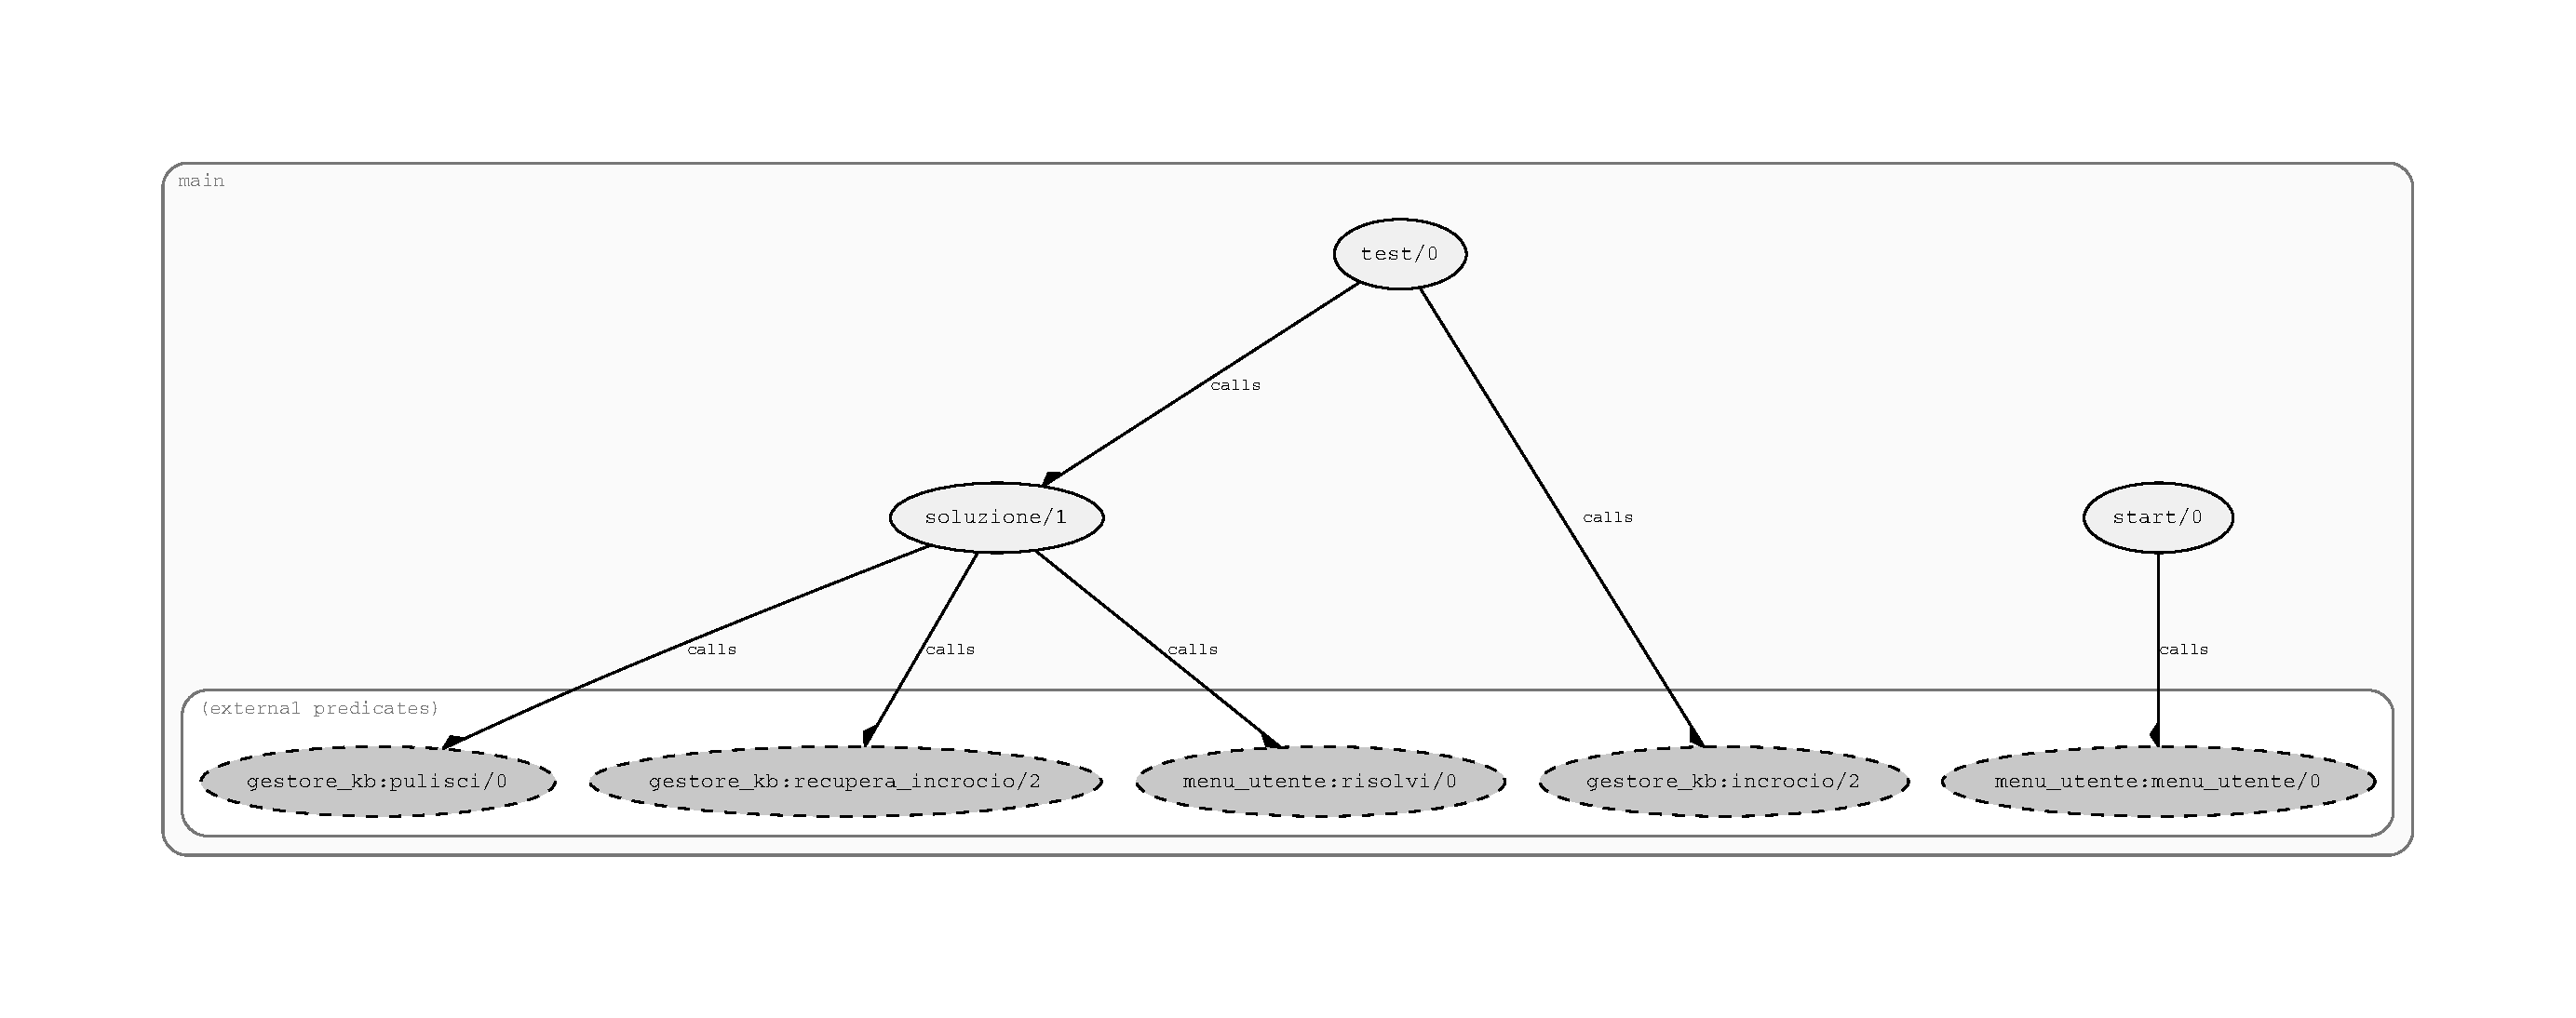
\includegraphics[scale=.5]{diagrams/main}}
	\caption{\texttt{main.pl}}
\end{figure}

\newgeometry{left=1cm, right=1cm, top=1mm, bottom=1mm}

\begin{sidewaysfigure}
	\thisfloatpagestyle{empty}
	\makebox[\textwidth]{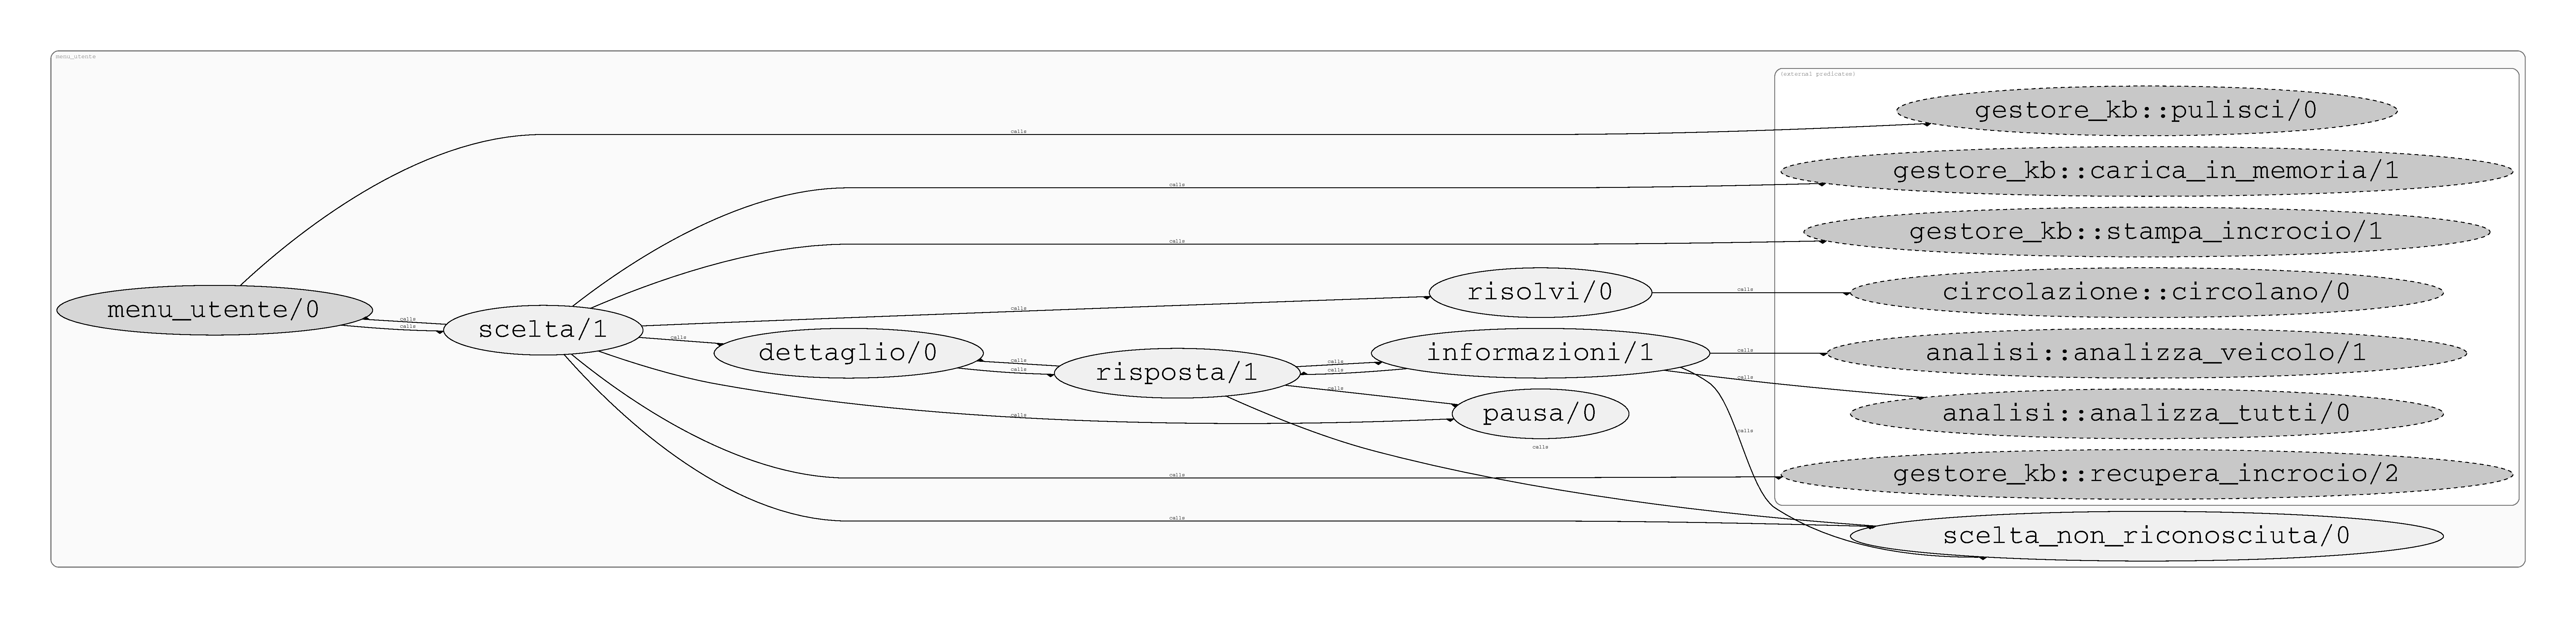
\includegraphics[scale=.2]{diagrams/menu_utente}}
	\caption{\texttt{menu\_utente.pl}}
\end{sidewaysfigure}

\begin{figure}
	\makebox[\textwidth]{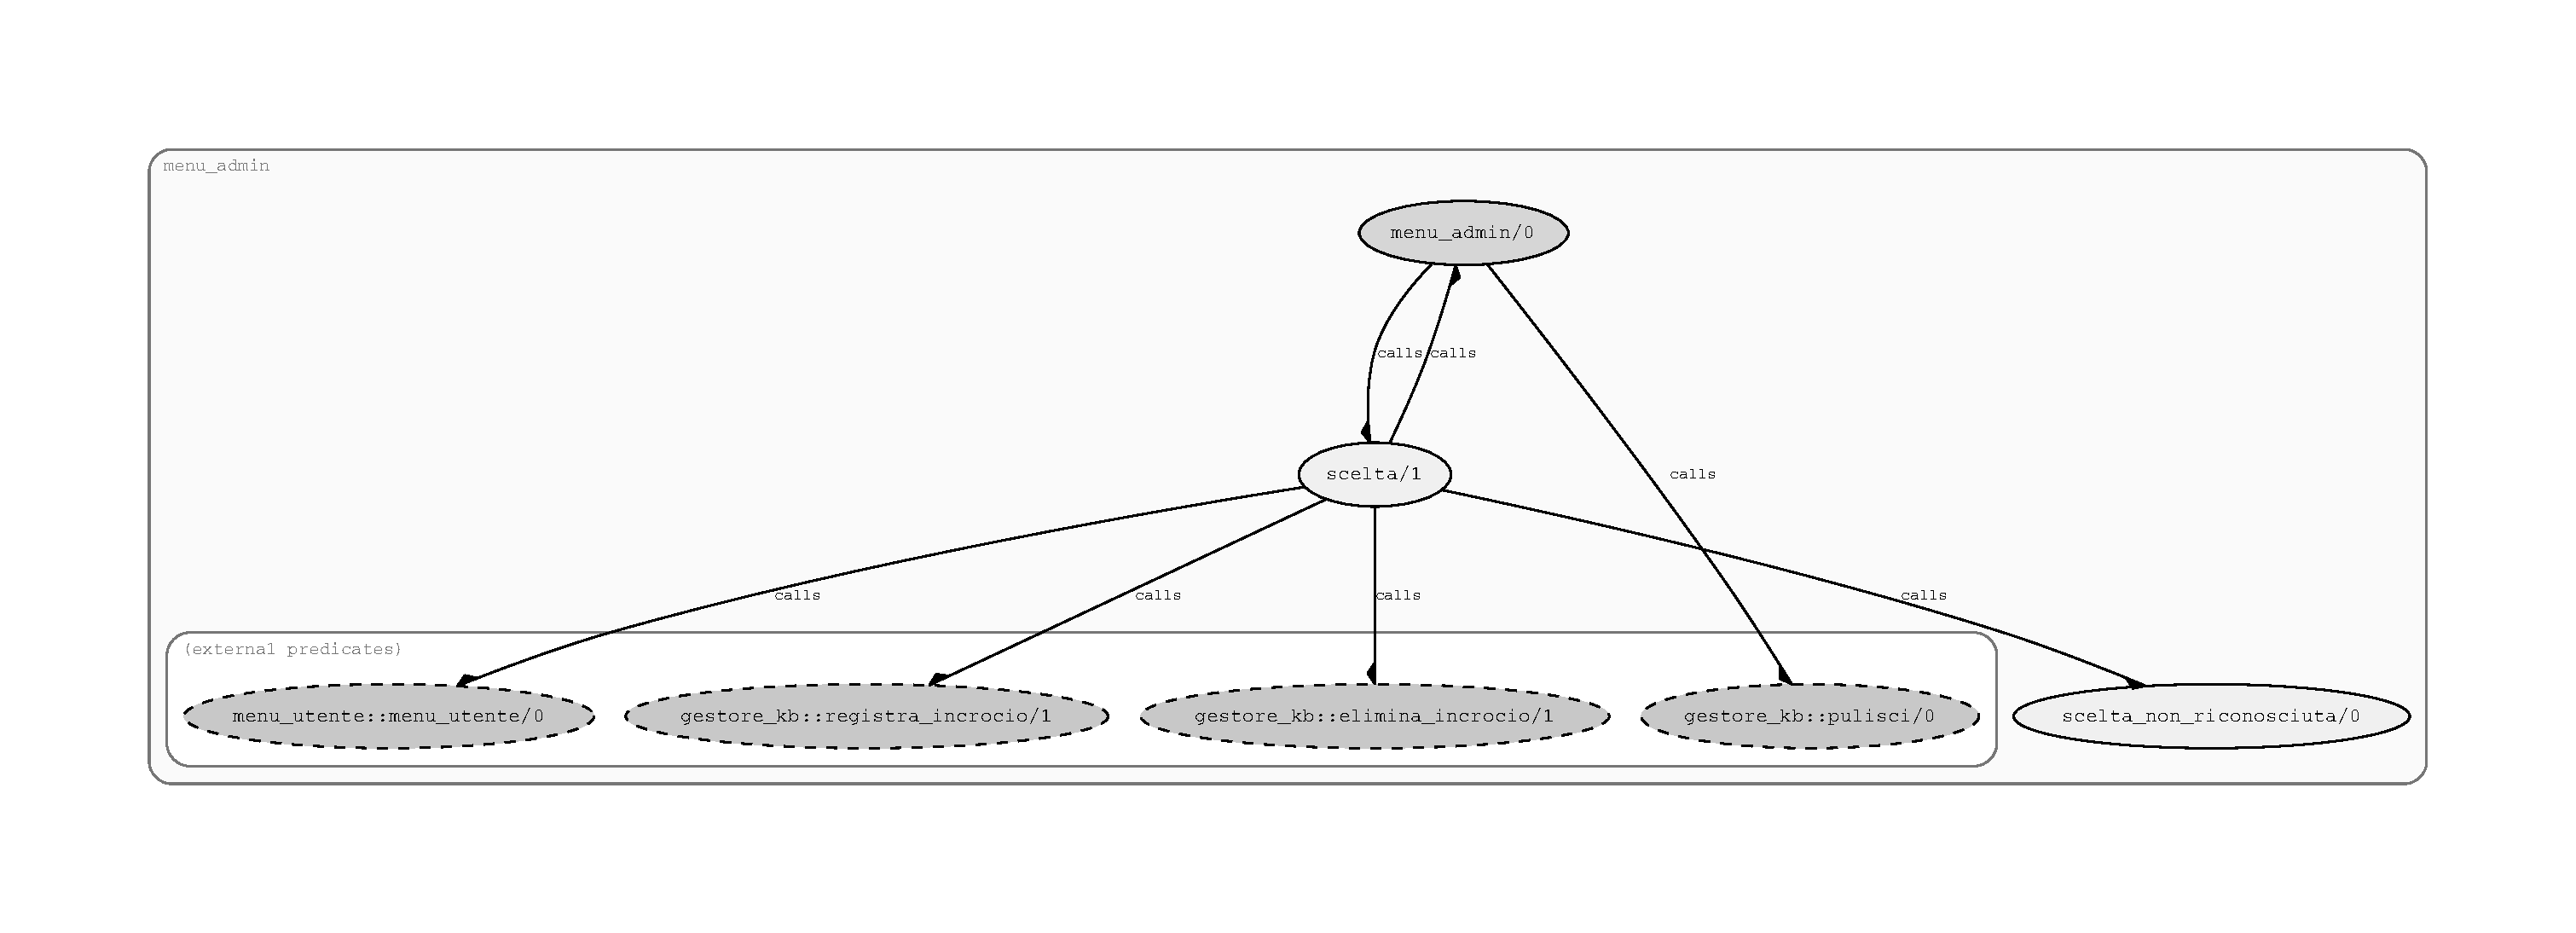
\includegraphics[width=1.2\textwidth]{diagrams/menu_admin}}
	\caption{\texttt{menu\_admin.pl}}
\end{figure}
\restoregeometry

\newgeometry{top=1mm, bottom=1mm, left=1mm, right=1mm}
\begin{sidewaysfigure}
	\thisfloatpagestyle{empty}
	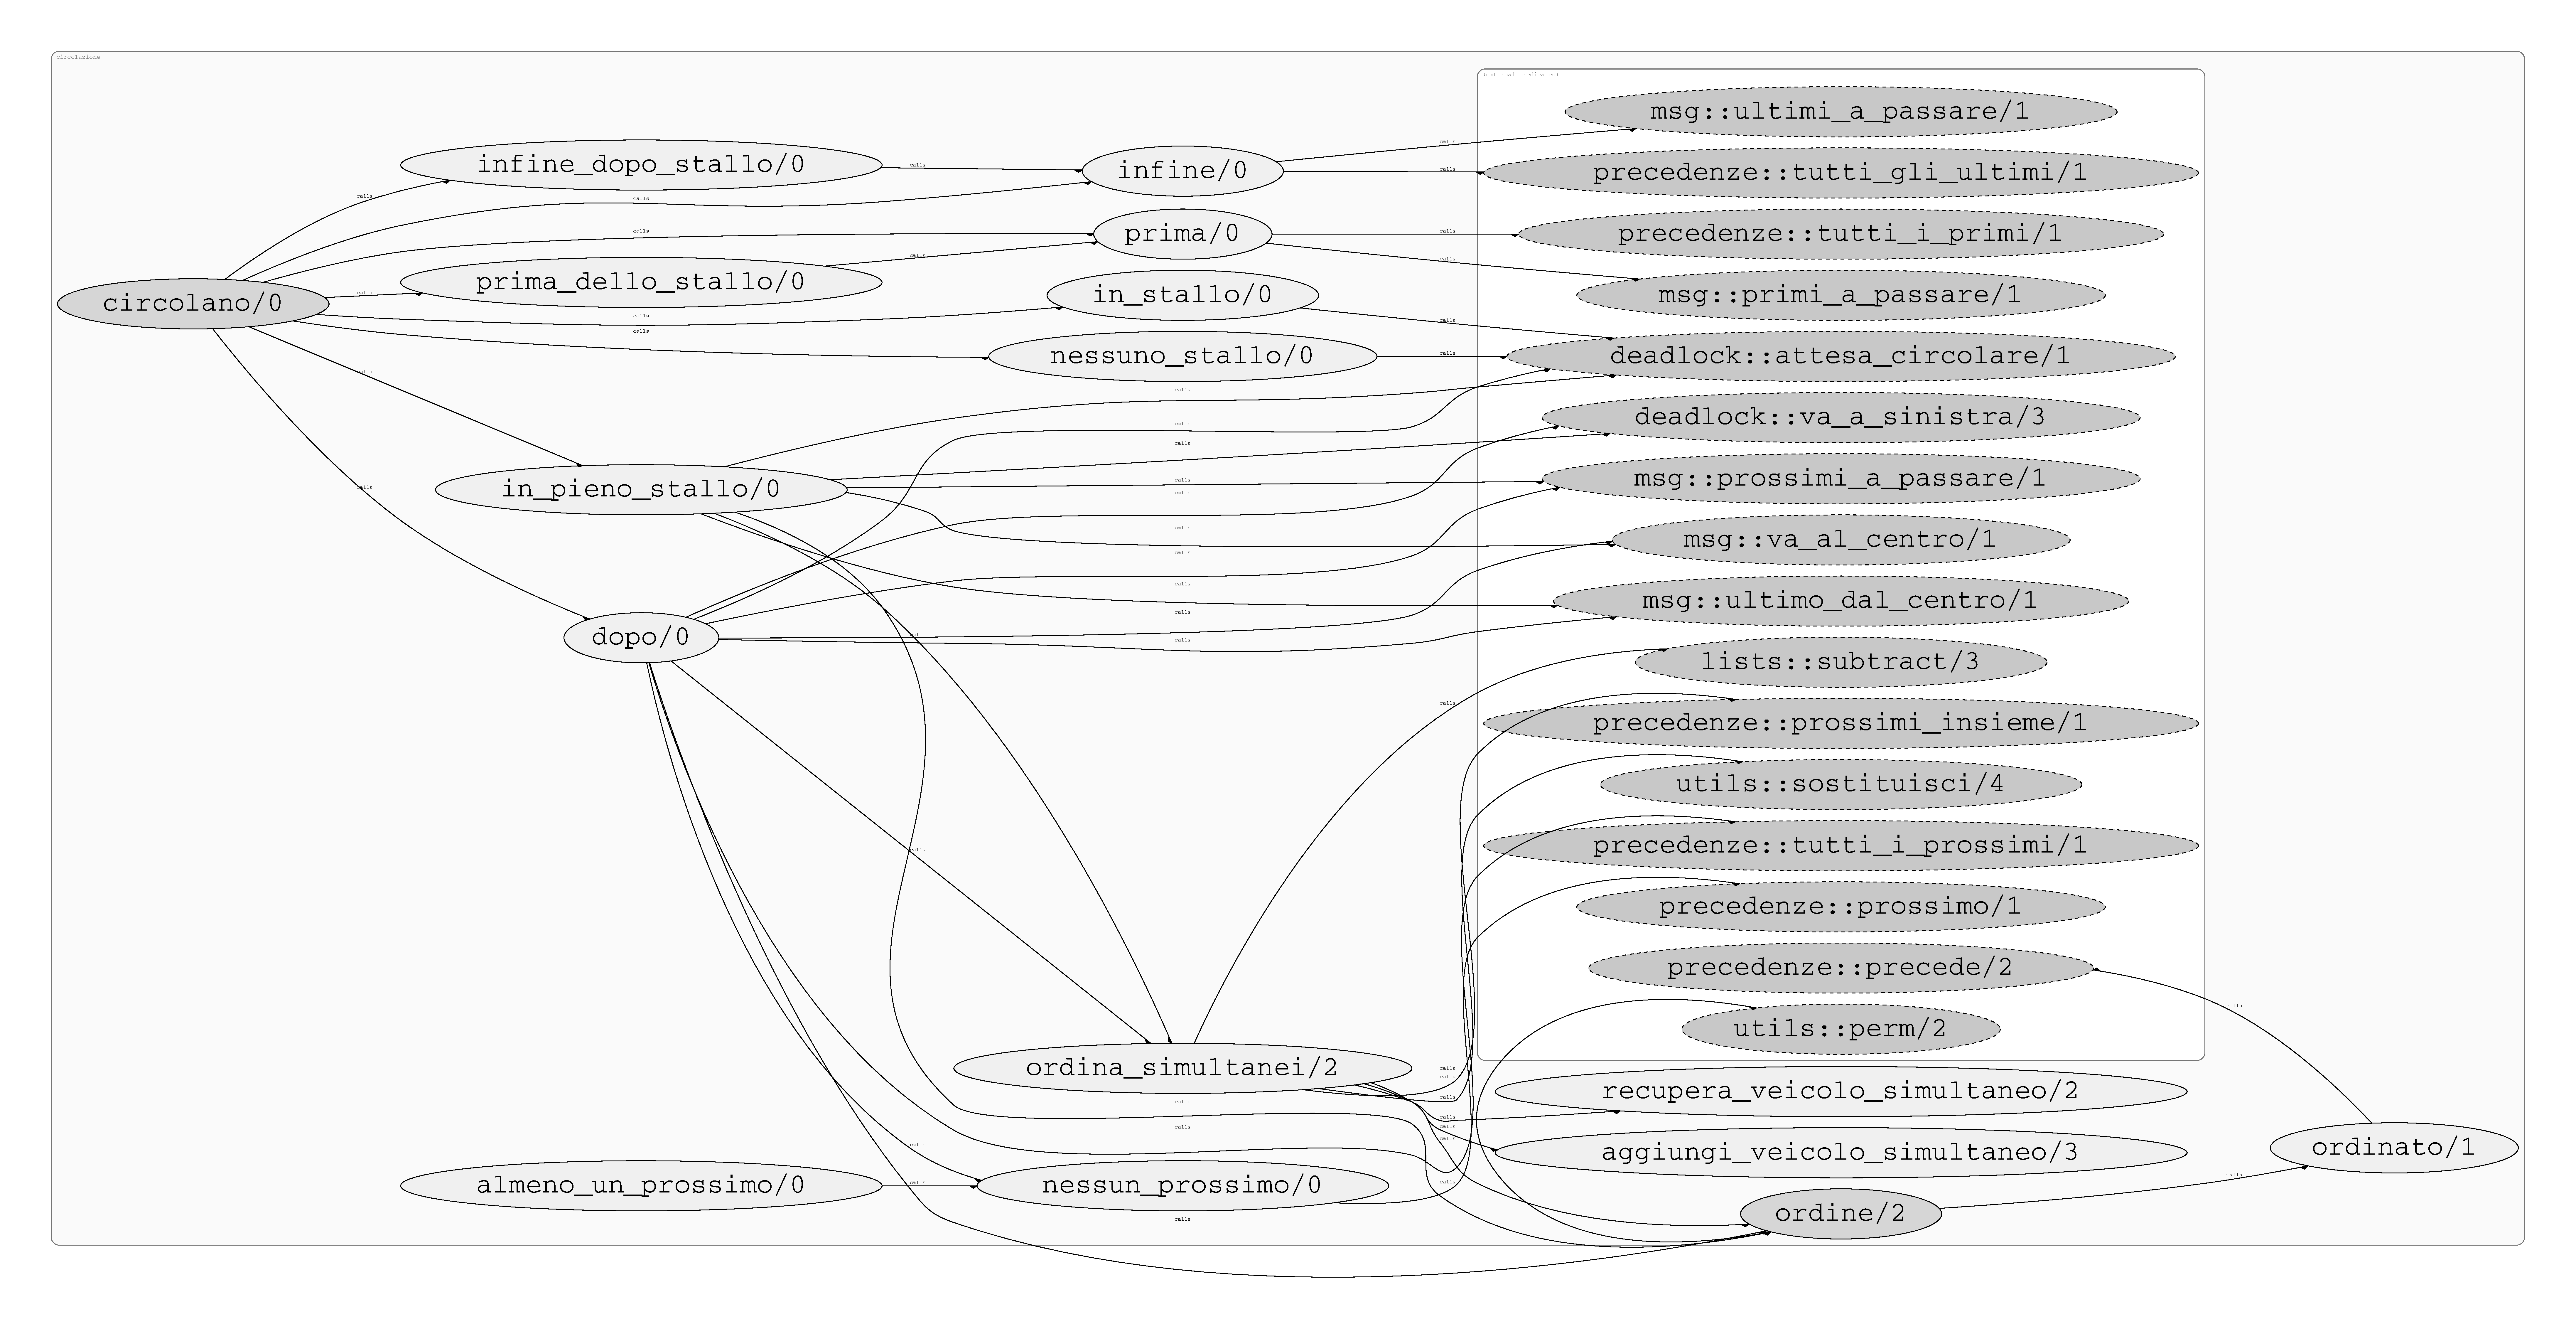
\includegraphics[width=\textwidth, height=\textheight, keepaspectratio]{diagrams/circolazione}
	\caption{\texttt{circolazione.pl}}
\end{sidewaysfigure}

\begin{sidewaysfigure}
	\thisfloatpagestyle{empty}
	
\includegraphics[width=\textwidth, height=\textheight, keepaspectratio]{diagrams/precedenze}
	\caption{\texttt{precedenze.pl}}
\end{sidewaysfigure}

\begin{sidewaysfigure}
	\thisfloatpagestyle{empty}
	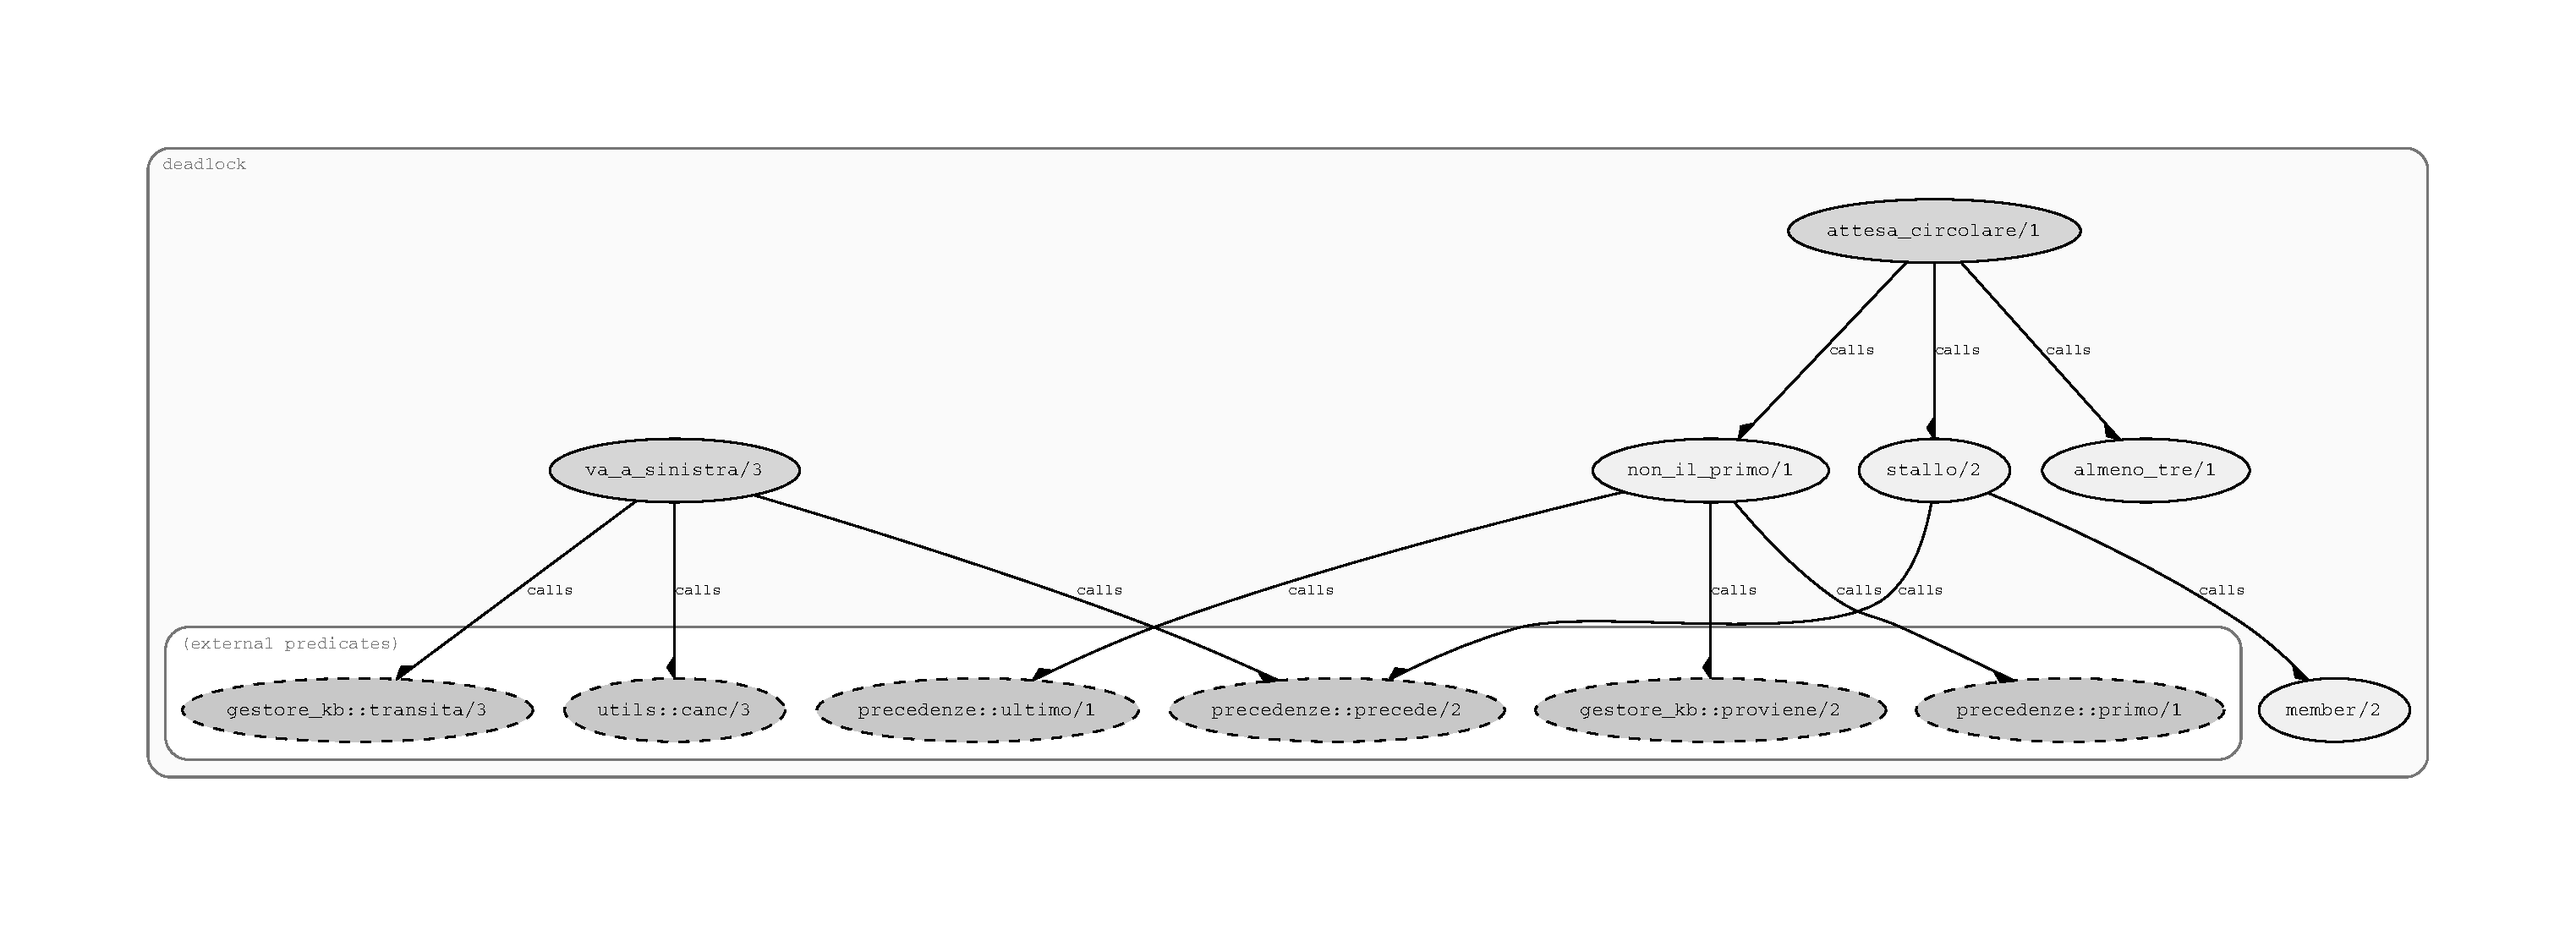
\includegraphics[width=\textwidth, height=\textheight, keepaspectratio]{diagrams/deadlock}
	\caption{\texttt{deadlock.pl}}
\end{sidewaysfigure}


\begin{figure}
	\makebox[\textwidth]{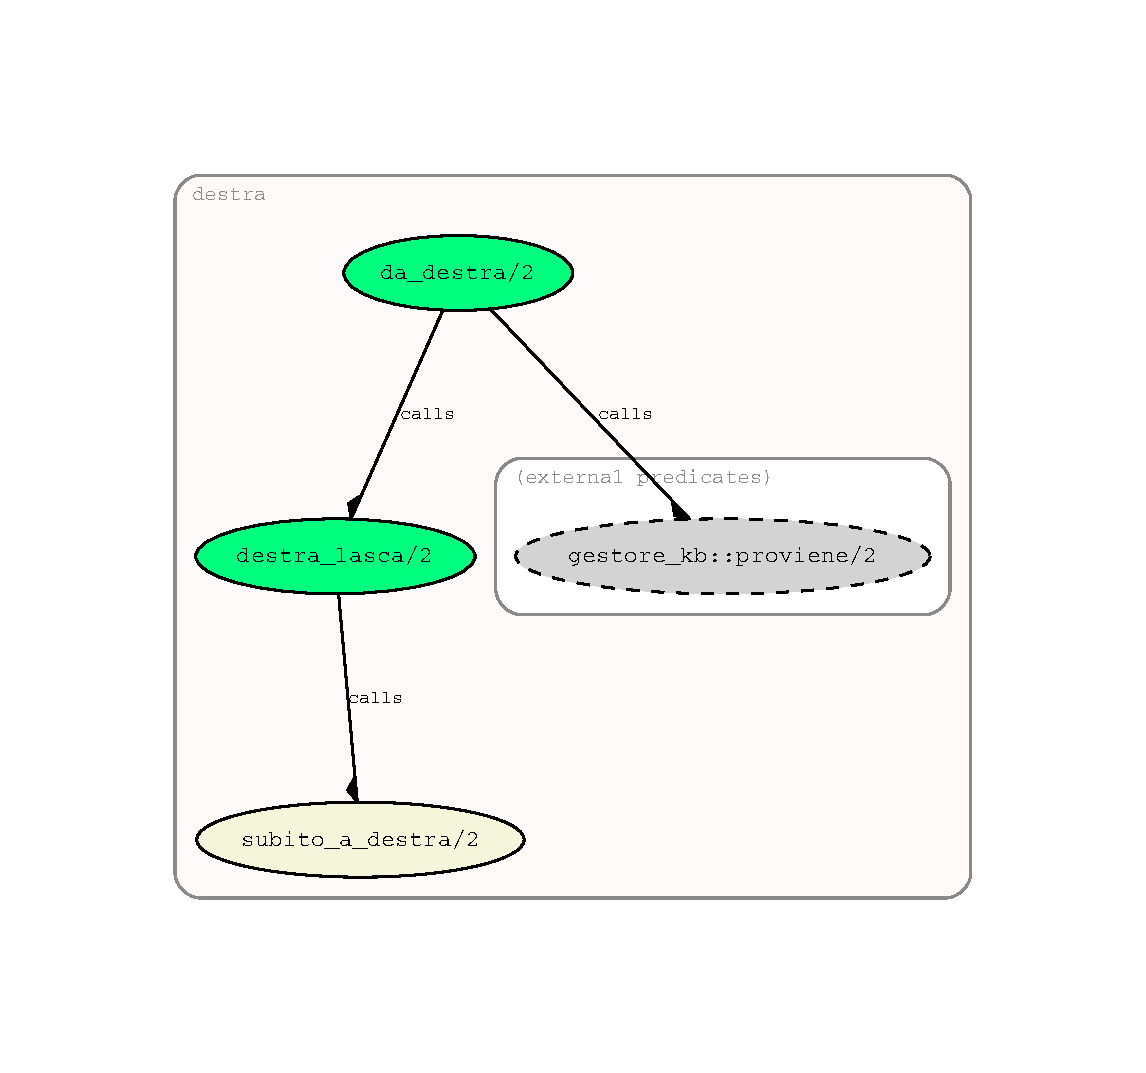
\includegraphics[width=1.2\textwidth]{diagrams/destra}}
	\caption{\texttt{destra.pl}}
\end{figure}

\begin{sidewaysfigure}
	\thisfloatpagestyle{empty}
	
\includegraphics[width=\textwidth, height=\textheight, keepaspectratio]{diagrams/analisi}
	\caption{\texttt{analisi.pl}}
\end{sidewaysfigure}

\begin{sidewaysfigure}
	\thisfloatpagestyle{empty}
	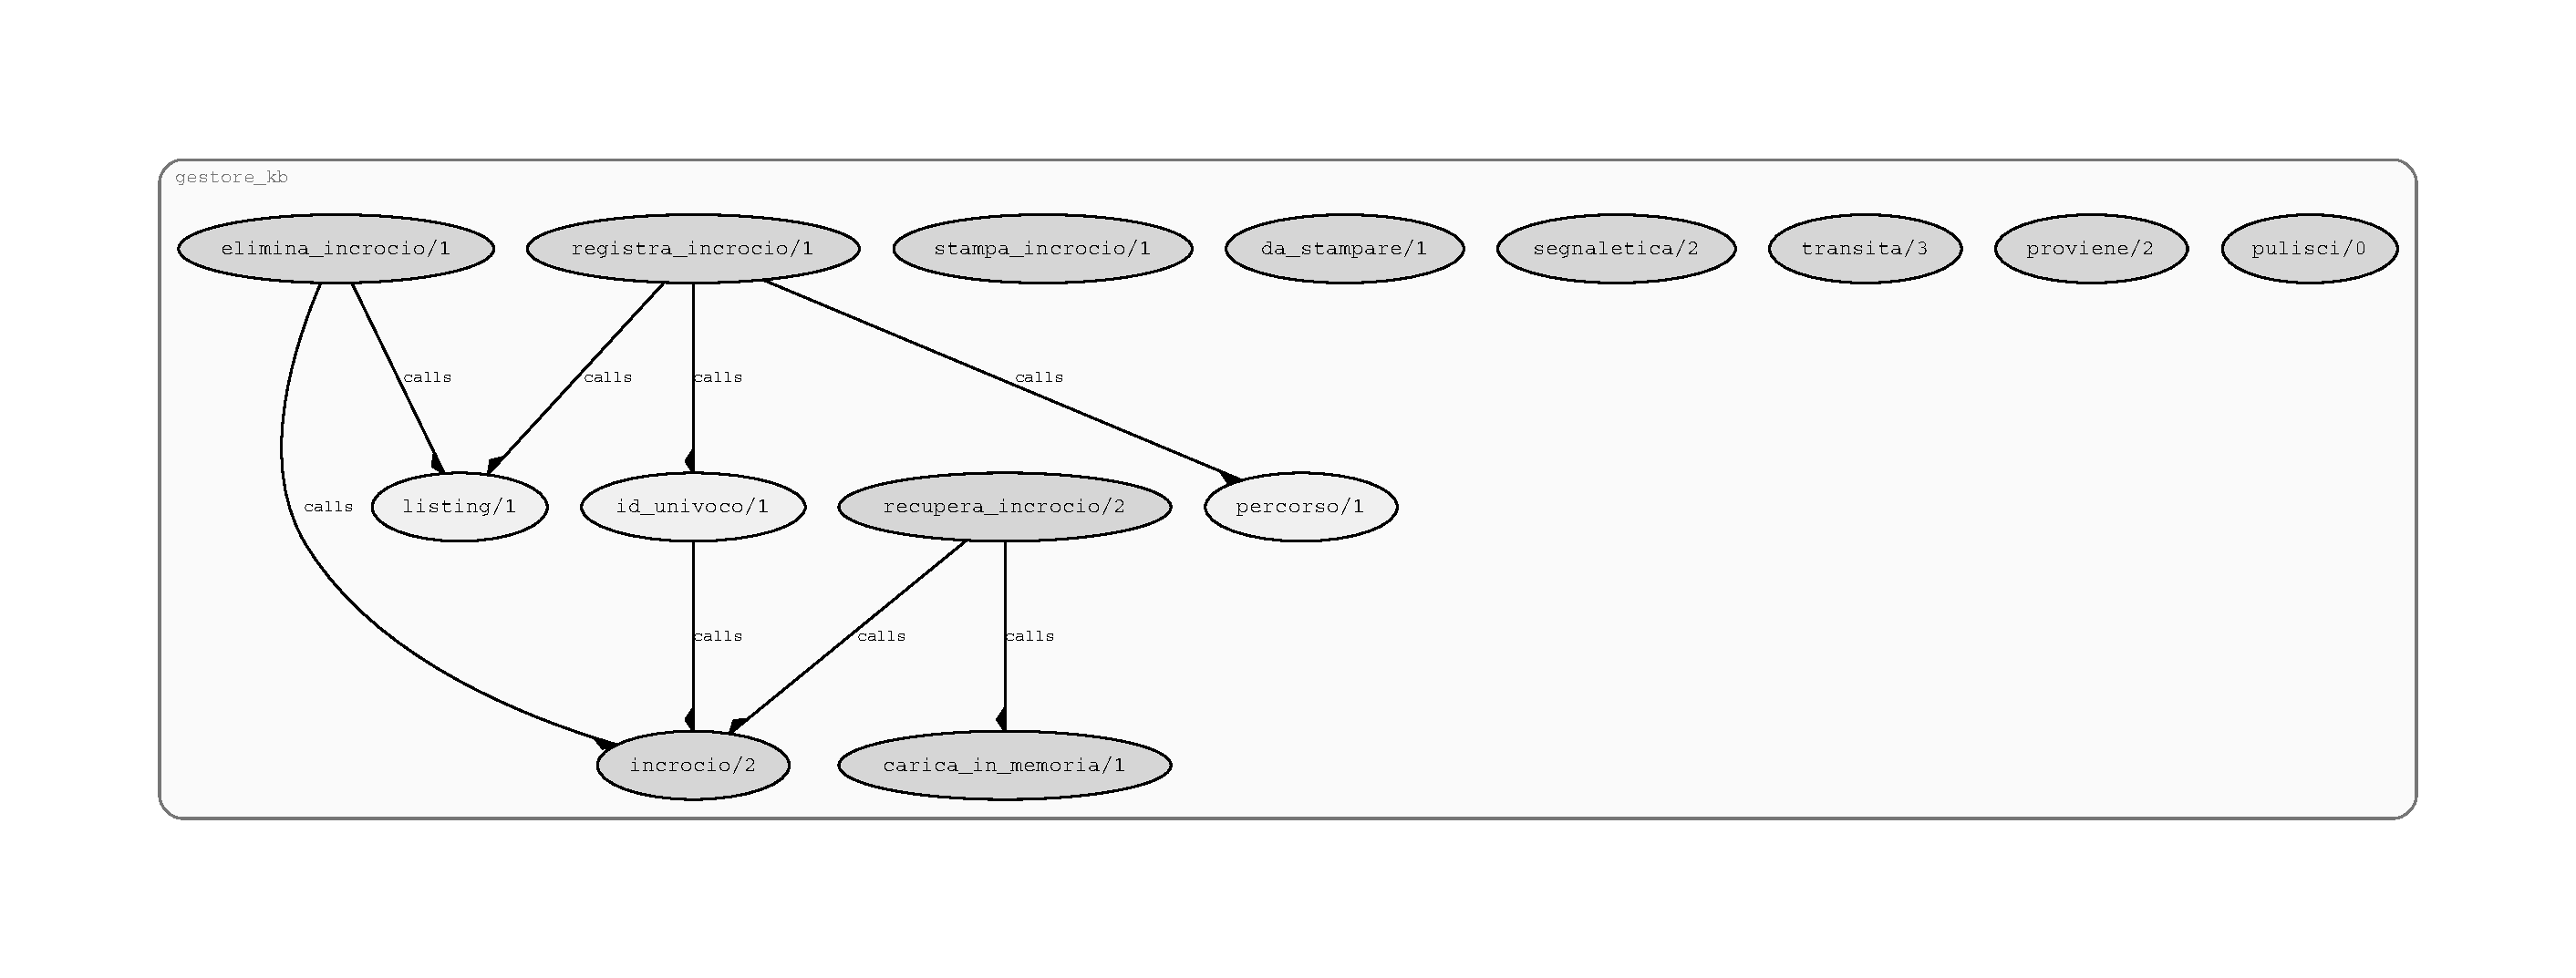
\includegraphics[width=\textwidth, height=\textheight, keepaspectratio]{diagrams/gestore_kb}
	\caption{\texttt{gestore\_kb.pl}}
\end{sidewaysfigure}

\begin{sidewaysfigure}
	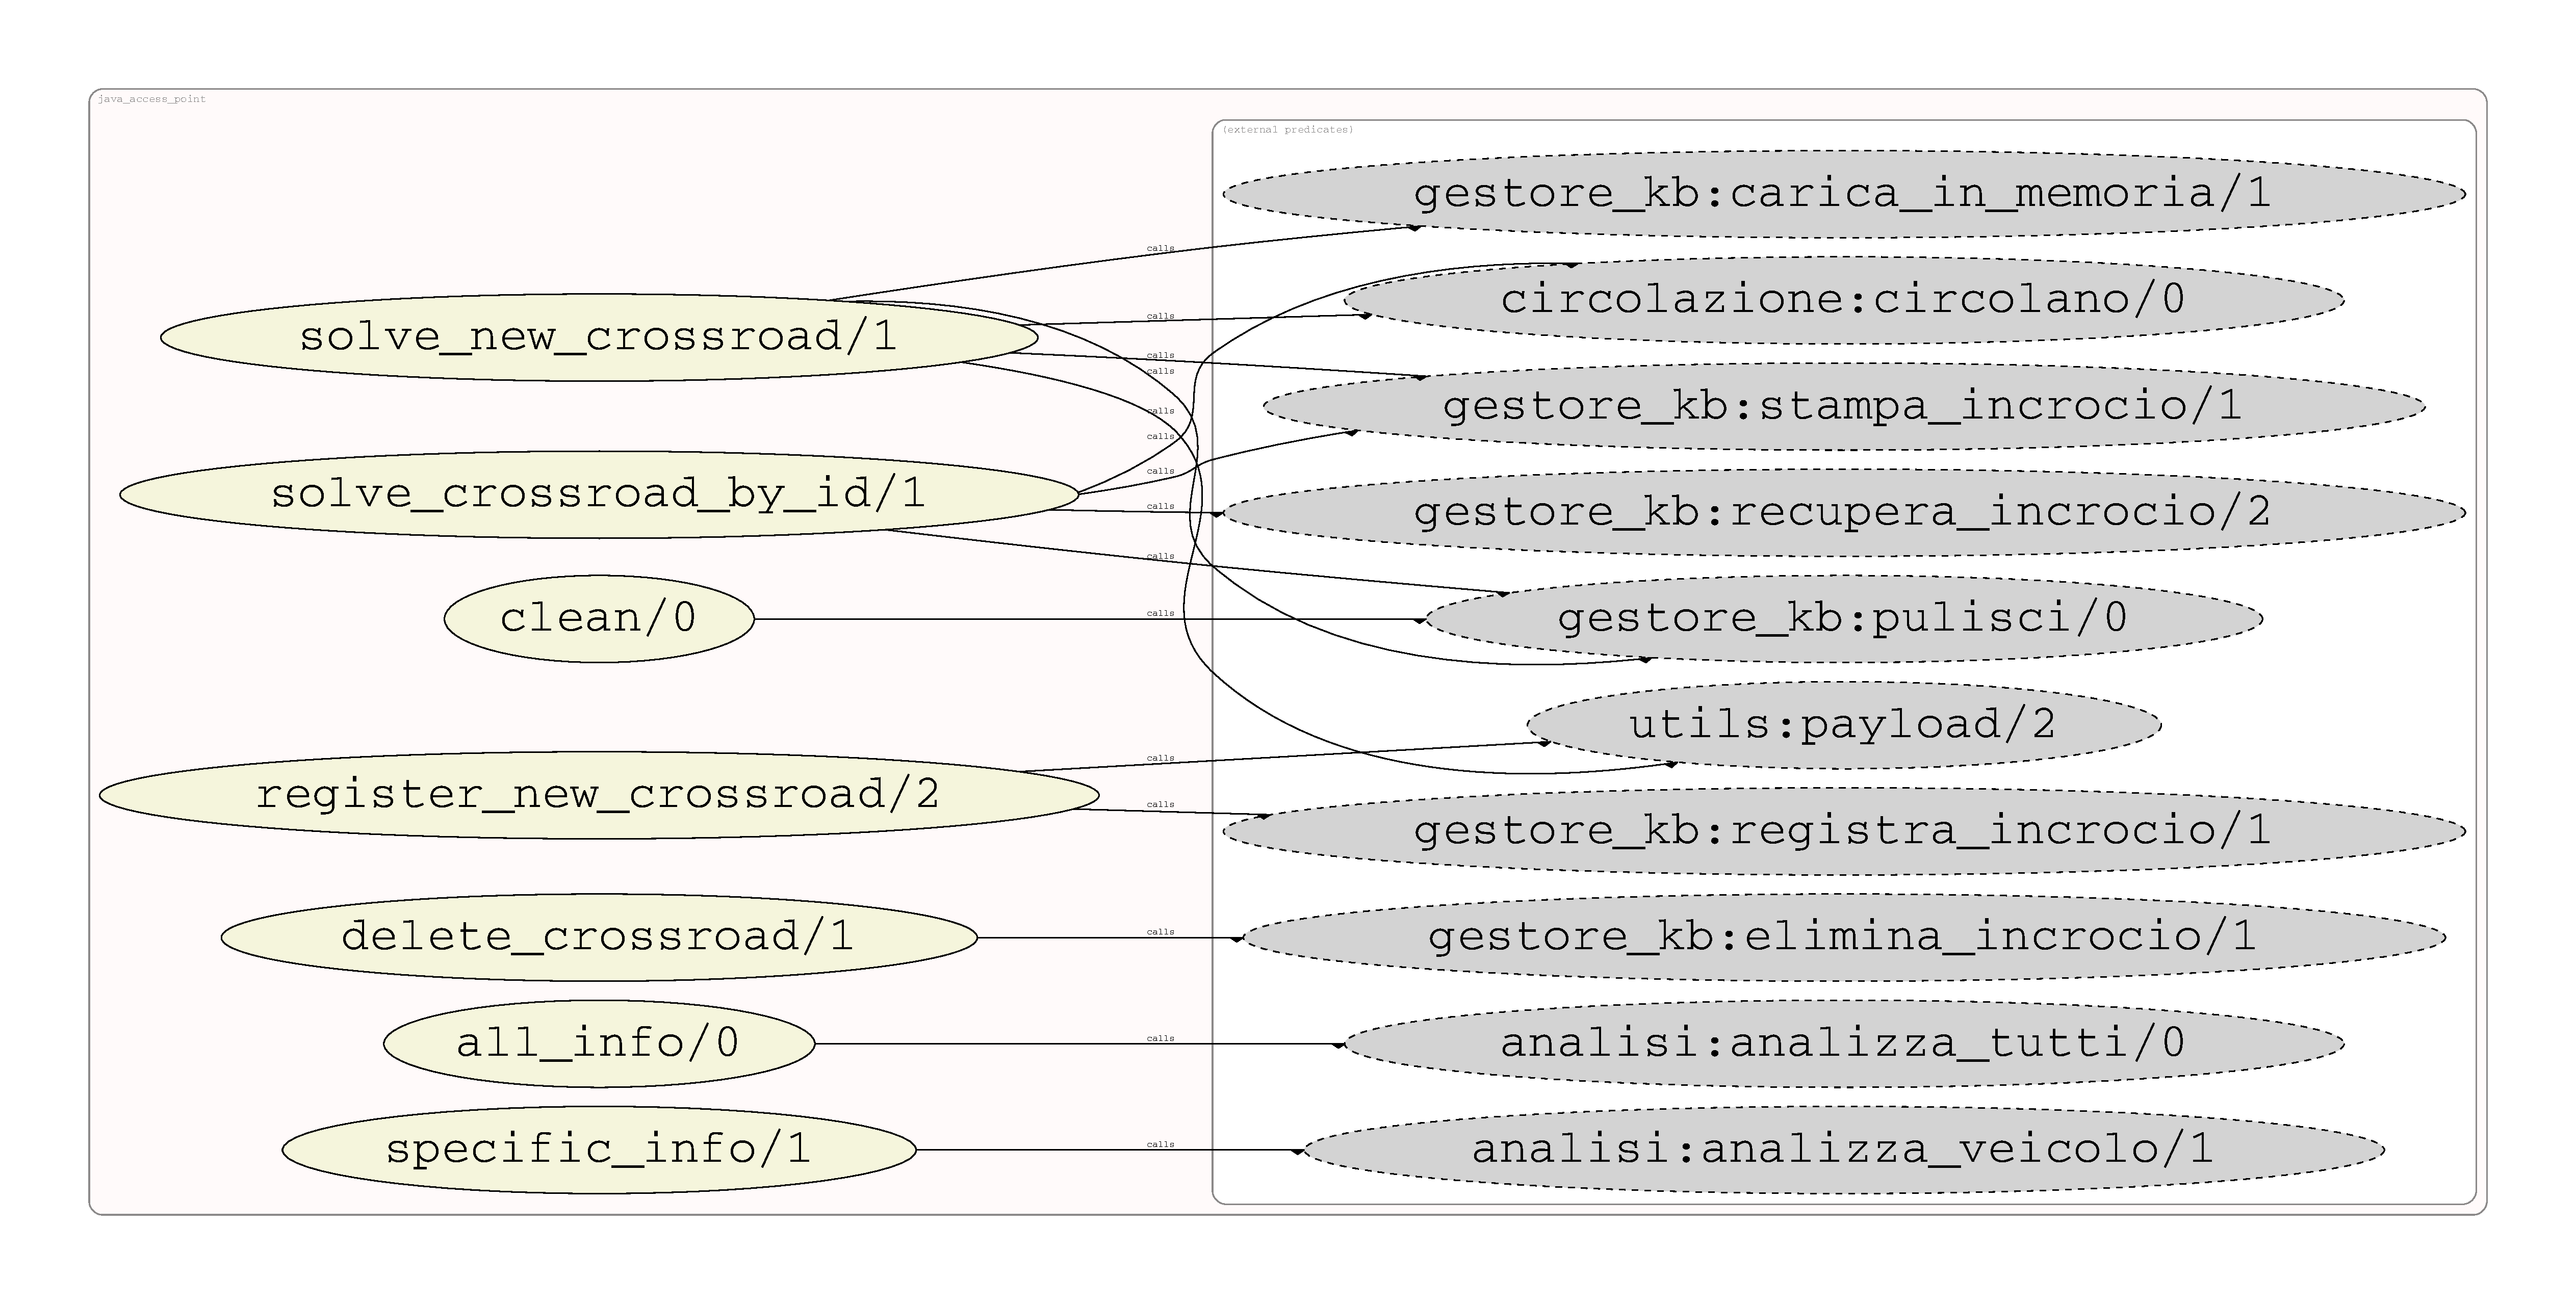
\includegraphics[width=\textwidth, height=\textheight, keepaspectratio]{diagrams/java_access_point}
	\caption{\texttt{java\_access\_point.pl}}
\end{sidewaysfigure}

\begin{figure}
	\centering
	\begin{subfigure}[b]{.4\textwidth}
		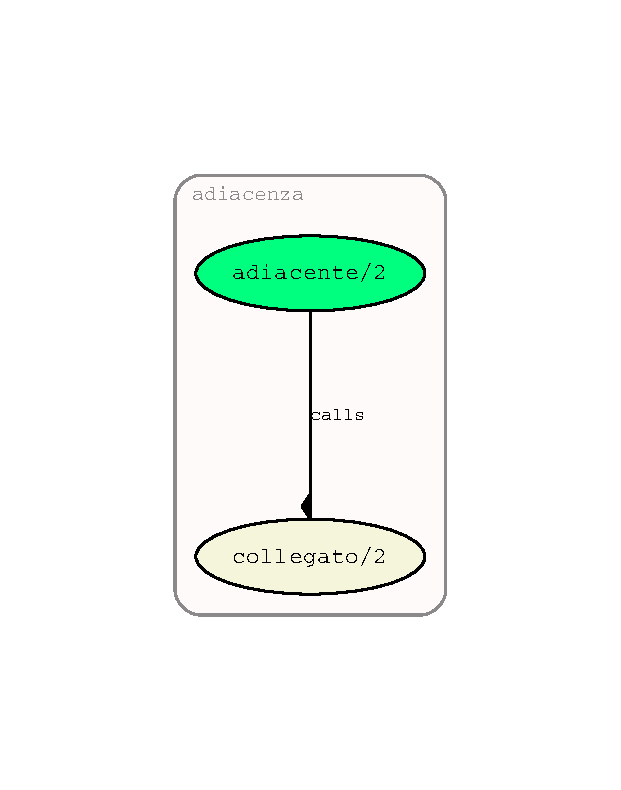
\includegraphics[width=\textwidth]{diagrams/adiacenza}
		\caption{\texttt{adiacenza.pl}}
	\end{subfigure}
	\begin{subfigure}[b]{.4\textwidth}
		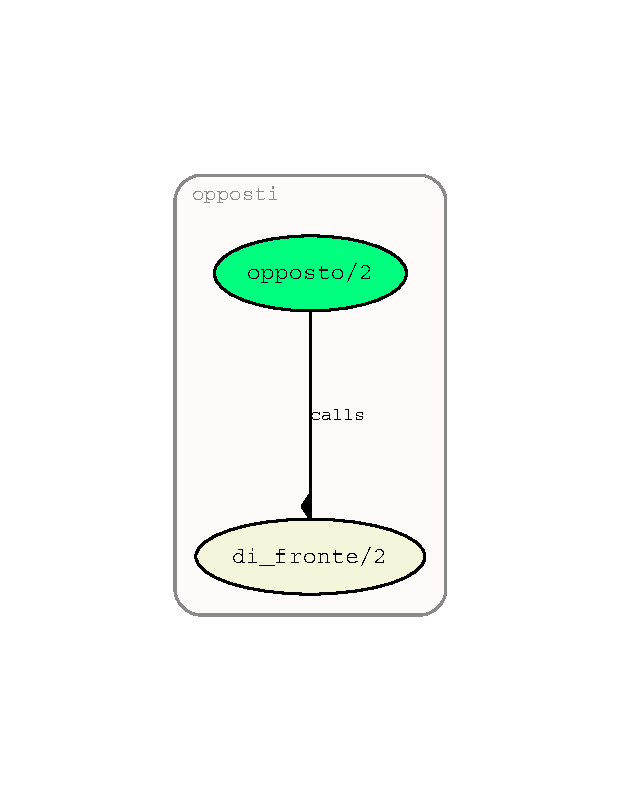
\includegraphics[width=\textwidth]{diagrams/opposti}
		\caption{\texttt{opposti.pl}}
	\end{subfigure}
	\begin{subfigure}[b]{.4\textwidth}
		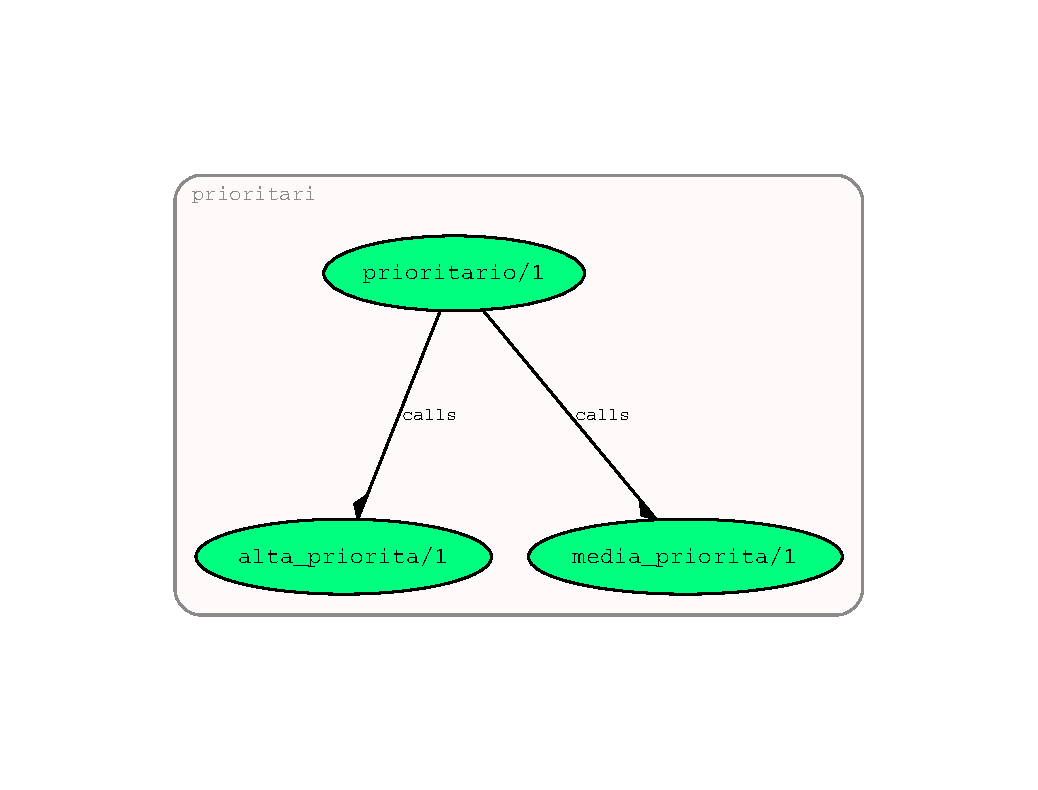
\includegraphics[width=\textwidth]{diagrams/prioritari}
		\caption{\texttt{prioritari.pl}}
	\end{subfigure}
	\begin{subfigure}[b]{.4\textwidth}
		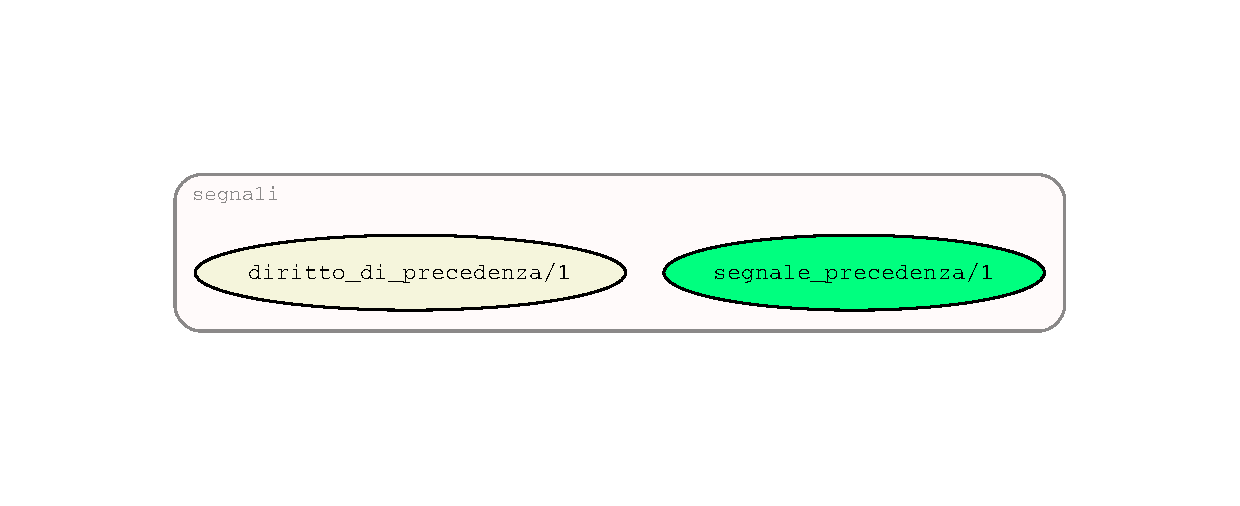
\includegraphics[width=\textwidth]{diagrams/segnali}
		\caption{\texttt{segnali.pl}}
	\end{subfigure}
\end{figure}

\begin{sidewaysfigure}
	
\includegraphics[width=\textwidth, height=\textheight, keepaspectratio]{diagrams/movimento}
	\caption{\texttt{movimento.pl}}
\end{sidewaysfigure}

\begin{sidewaysfigure}
	\thisfloatpagestyle{empty}
	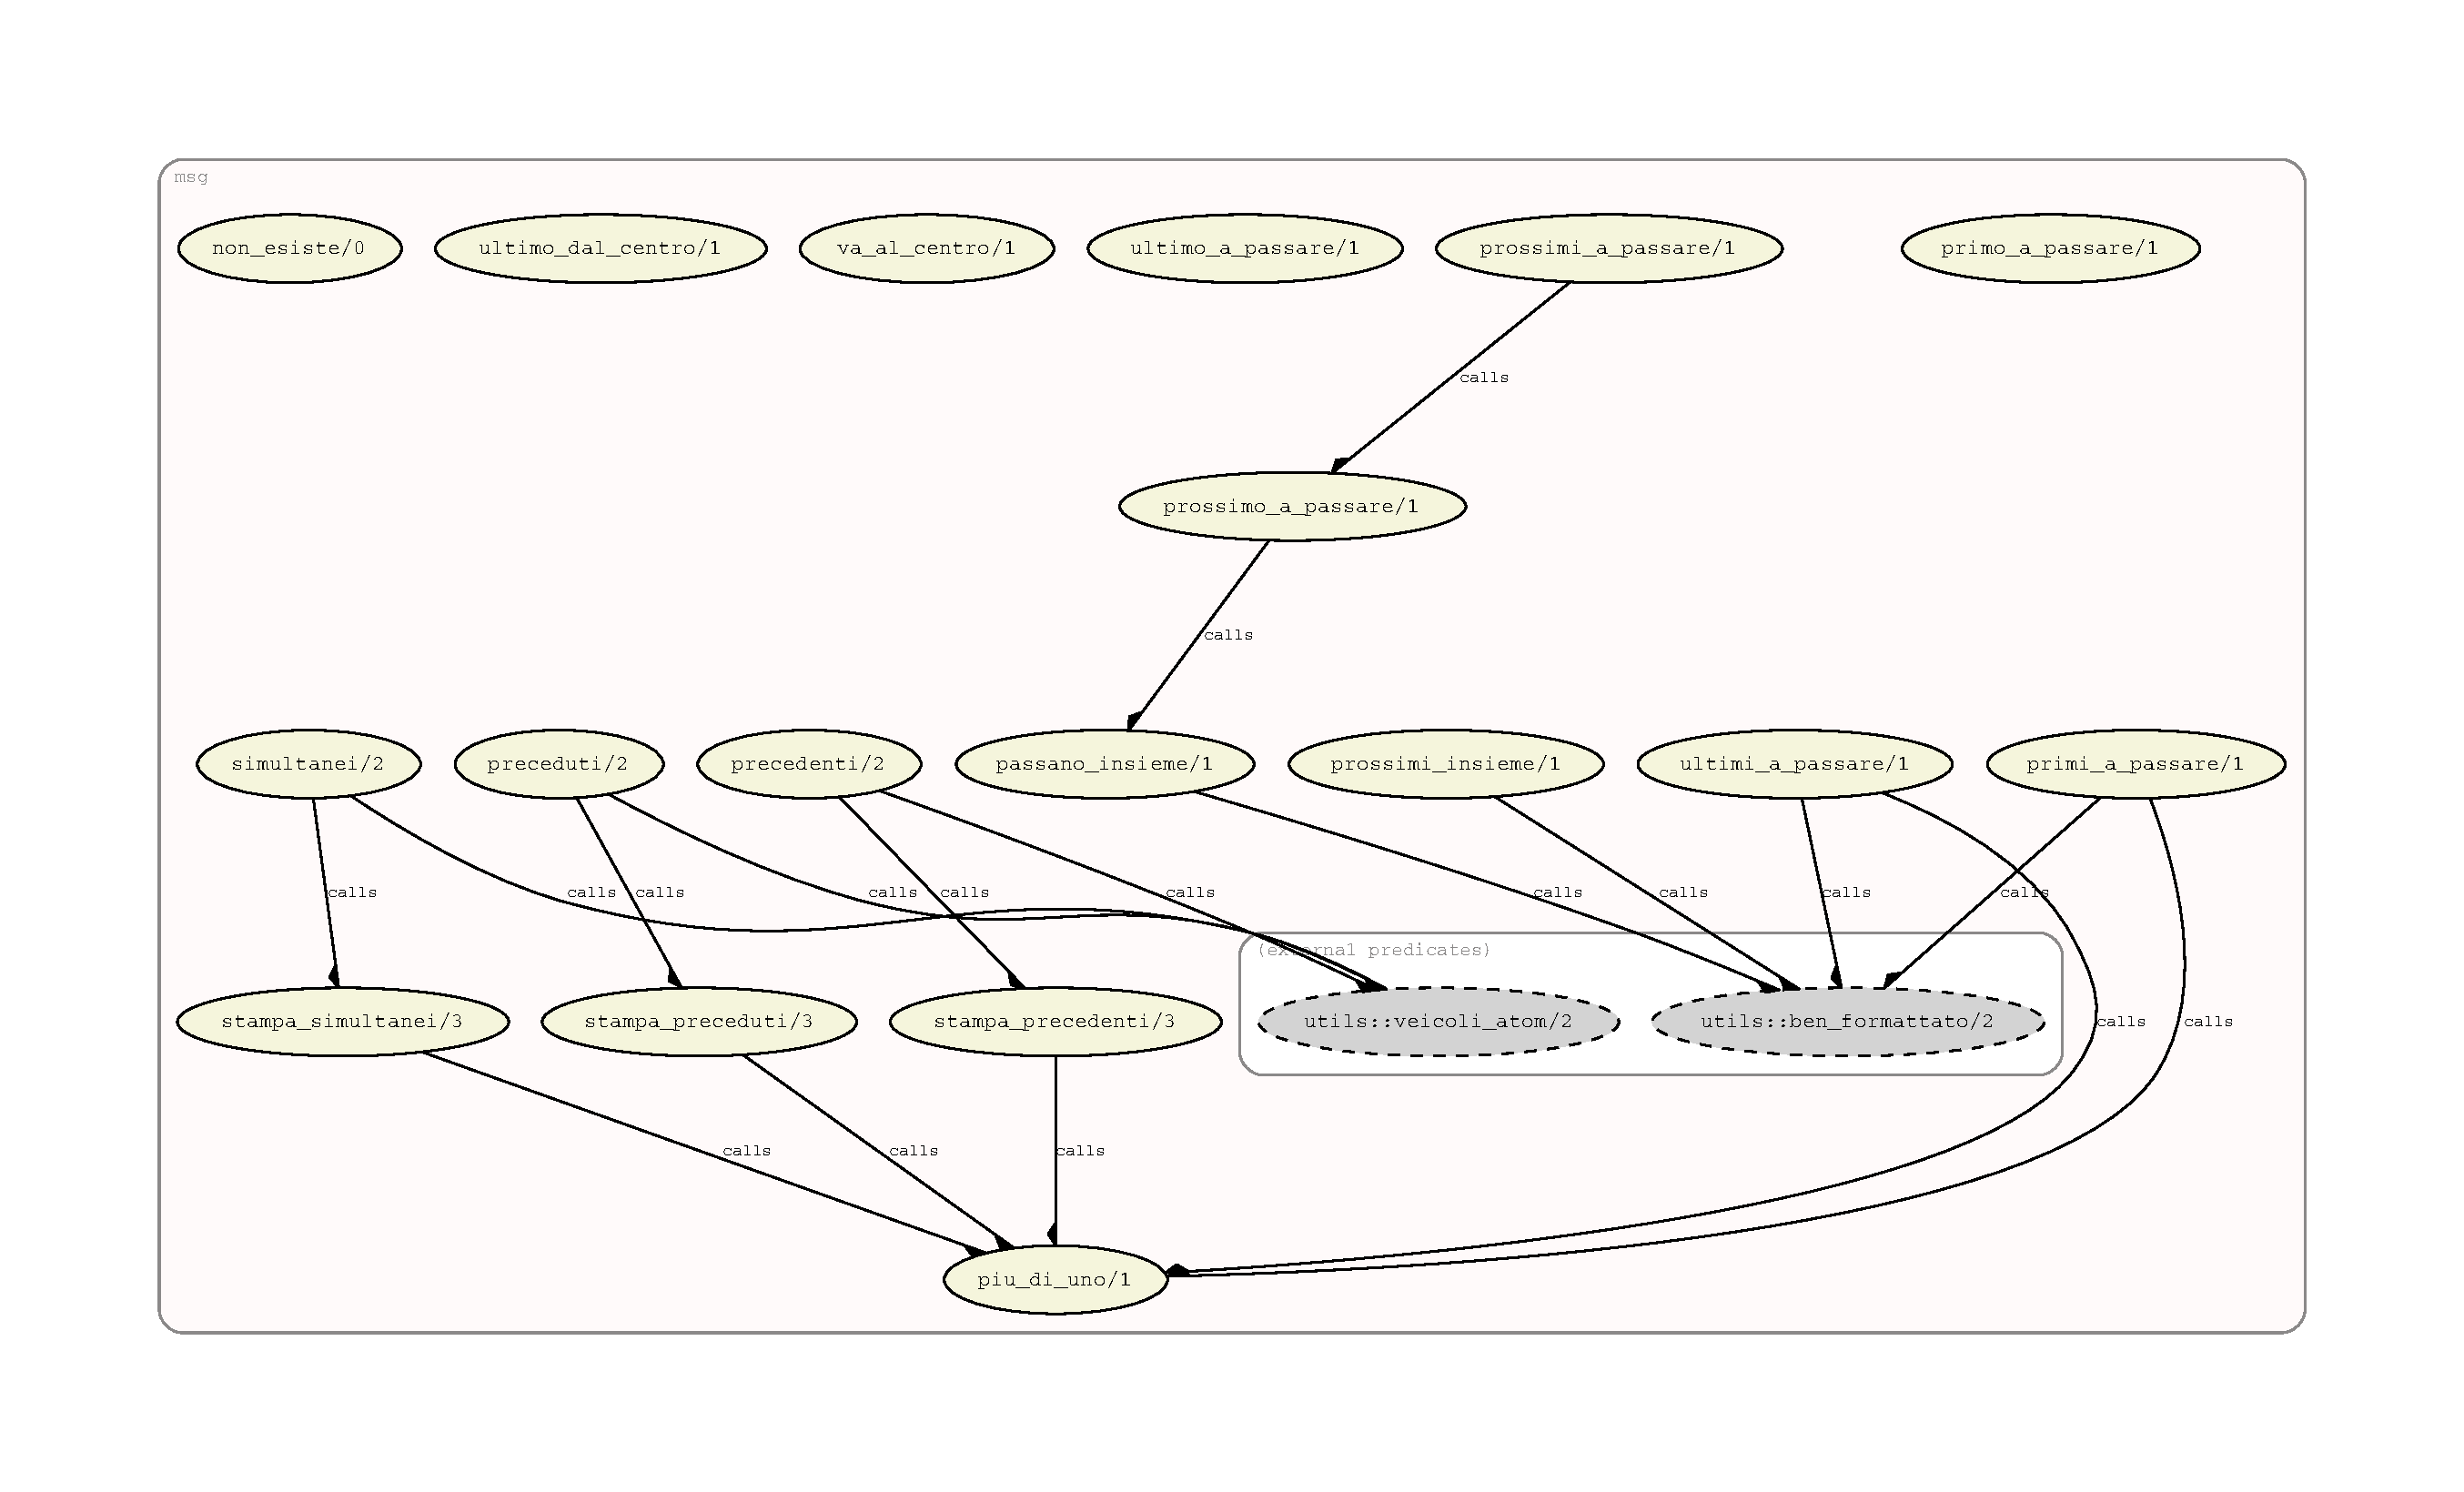
\includegraphics[width=\textwidth, height=\textheight, keepaspectratio]{diagrams/msg}
	\caption{\texttt{msg.pl}}
\end{sidewaysfigure}

\begin{sidewaysfigure}
	\thisfloatpagestyle{empty}
	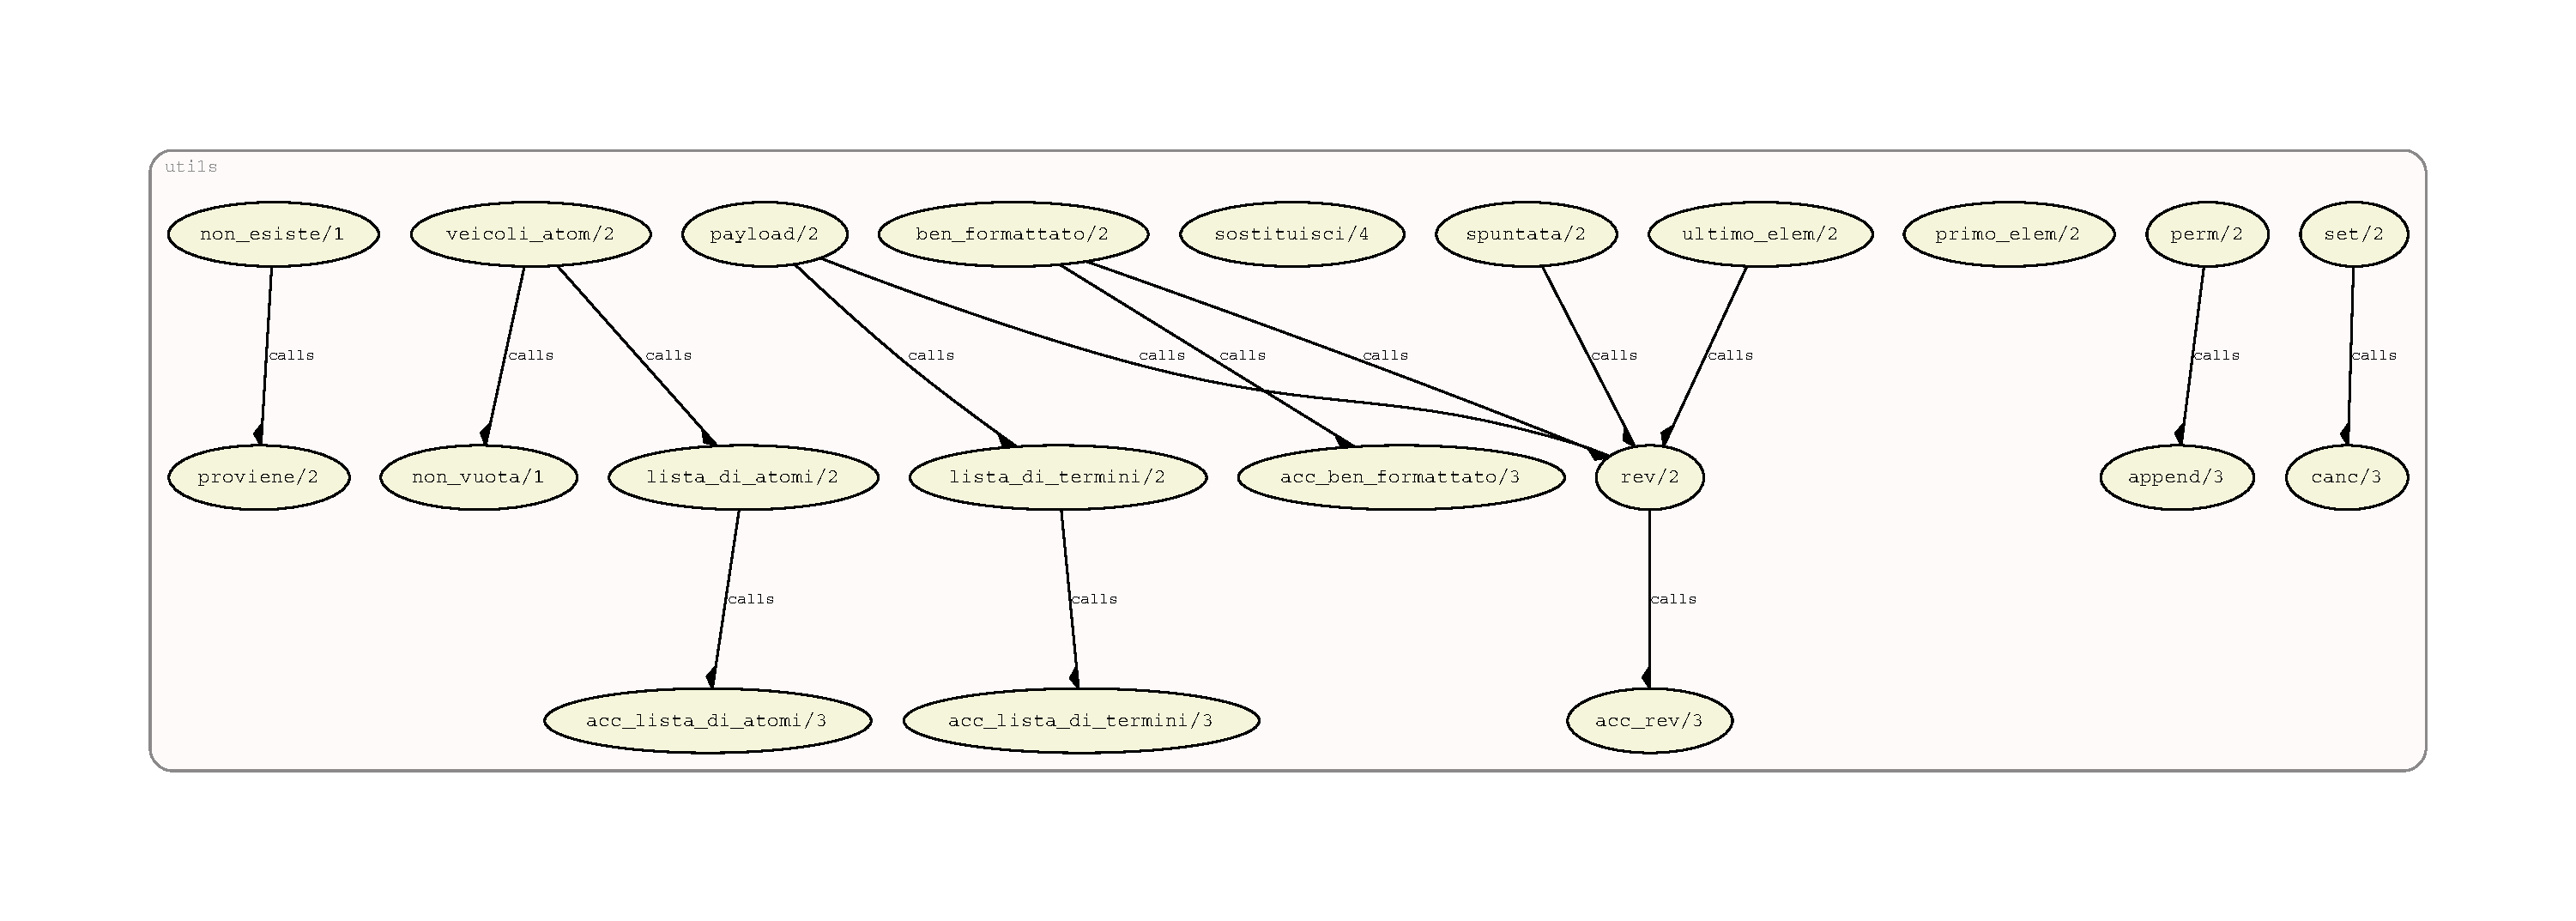
\includegraphics[width=\textwidth, height=\textheight, keepaspectratio]{diagrams/utils}
	\caption{\texttt{utils.pl}}
\end{sidewaysfigure}

\restoregeometry

\section{Ordine dei veicoli}
È importante capire come i veicoli possano circolare ordinatamente, in un incrocio a scorrimento normale o in presenza di uno stallo.

\subsection{Precedenza}
Visti i casi espressi in \ref{ssec:prec}, descriviamo i passaggi che prevedono l'utilizzo di \texttt{precede/2} nel file \texttt{precedenze.pl}. Come è ovvio, il predicato \texttt{precede/2} prende due argomenti, i due veicoli, e verifica se esiste un diritto di precedenza per l'uno o per l'altro. Esistono varie situazioni in cui questi veicoli possono trovarsi:
\begin{enumerate}
	\item I due veicoli sono prioritari, quindi bisogna controllare chi la ``spunta":
		\begin{itemize}
			\item Uno ha la priorità più alta, quindi gode della precedenza sull'altro (per esempio, ambulanza su tram).
			\item I due hanno la stessa priorità, quindi si applicano le normali regole di precedenza.
		\end{itemize}
	\item Un veicolo è prioritario e l'altro no: il primo ha la precedenza.
	\item Due veicoli sono ordinari (non prioritari):
		\begin{itemize}
			\item Se non ci sono segnali, si applicano le regole del CdS.
			\item Se uno è soggetto ad un segnale, l'altro ha la precedenza.
			\item Se entrambi sono soggetti ad un segnale, gli eventuali altri veicoli presenti nell'incrocio hanno la precedenza, infine si applicano le normali regole di precedenza per entrambi.
		\end{itemize}
\end{enumerate}

Una volta inquadrato il caso tra quella elencati sopra, l'effettiva precedenza tra due veicoli viene affrontata da altri due predicati, \texttt{precede\_da\_destra/2} e \texttt{precedenza\_frontale/2}. Il primo verifica che un veicoli provenga da destra e che \textbf{incroci} l'altro, il secondo implementa esattamente i casi visti in \ref{sssec:front}. Il predicato \texttt{incrocia/2} indica quando un veicolo entra in contatto con un altro durante la sua manovra. Il suo uso viene descritto meglio in \ref{ssec:pos} dove si parla del modulo in cui è contenuto.

\subsection{Circolazione}
I modelli di circolazione sono due, come visto in \ref{ssec:circ}, che di fatto vengono descritti da due regole:

\begin{verbatimtab}
circolano :-
	nessuno_stallo,
	prima,
	dopo,
	infine.

circolano :-
	in_stallo,
	prima_dello_stallo,
	in_pieno_stallo,
	infine_dopo_stallo.
\end{verbatimtab}

La prima clausola di \texttt{circolano/0} descrive il primo caso, quello in cui non ci sono stalli e ricostruisce l'ordine corretto di transito dei veicoli. La seconda clausola, invece, accerta l'esistenza di uno stallo e procede a ritrovare quali veicoli passano prima di esso, entrando poi nel merito cercando di risolverlo ed infine verifica se ci sono altri veicoli che passano per ultimi.

\subsection{Sorting}
Questa sezione entra nel dettaglio di quanto già detto in \ref{ssec:circ}, per descrivere l'algoritmo di ordinamento. È stato implementato un \emph{na\"{\i}ve sort}\cite{Clocksin:2003}, presente nel modulo \texttt{circolazione.pl}, così formato:
\begin{verbatimtab}
ordine(Lista, Ordinata) :-
	utils:perm(Lista, Ordinata),
	ordinato(Ordinata).

ordinato([]).

ordinato([_]).

ordinato([X,Y|T]) :-
	precede(X,Y),
	ordinato([Y|T]).
\end{verbatimtab}

Il predicato \texttt{ordine/2} verifica che una qualche permutazione della lista dei veicoli (ottenuta da \texttt{utils:perm/2}) è ordinata. Se non è così, ne viene generata un'altra. Il predicato \texttt{ordinato/1} dice che una lista è ordinata se è vuota, ha un solo veicolo o ogni veicolo precede il successivo nella lista.
\\\\
La permutazione avviene utilizzando \texttt{perm/2} presente nel modulo \texttt{utils.pl:}
\begin{verbatimtab}
perm([], []).
	
perm(L, [H|PermutRimanenti) :-
	append(V, [H|U], L),
	append(V, U, W),
	perm(W, PermutRimanenti).
\end{verbatimtab}

L'idea alla base di \texttt{perm/2} è che una permutazione della lista ha come elemento la testa della lista che è seguita da una permutazione degli elementi rimanenti della stessa.

\subsection{Stallo}
Riprendiamo ciò che è stato detto in \ref{sssec:lock}, quando alcuni veicoli si ritrovano a dover dare ed avere precedenza in cerchio, senza che nessuno passi per prima, apparentemente. Per verificare se ci sia o meno una situazione di stallo, ci viene in soccorso il predicato \texttt{attesa\_circolare/1} presente nel modulo \texttt{deadlock.pl}:

\begin{verbatimtab}
attesa_circolare(Veicoli) :-
	setof(V, non_il_primo(V), Veicoli),
	almeno_tre(Veicoli),
	stallo(Veicoli, Veicoli).
\end{verbatimtab}

Esso recupera una lista di veicoli non primi (ottenuti grazie all'operatore \texttt{setof/3}) che contenga almeno tre elementi. Una volta scoperti questi veicoli, si verifica se esiste o meno uno stallo:
\begin{verbatimtab}
stallo([H|T], Veicoli) :-
	precede(Precede, H),
	member(Precede, Veicoli),
	stallo(T, Veicoli).

stallo([], _).
\end{verbatimtab}

Il predicato \texttt{stallo/2} verifica che il veicolo in testa alla lista sia preceduto da un veicolo che faccia parte della lista, e si continua così per tutti gli altri veicoli.

\subsection{Veicoli simultanei}
Può capitare che un gruppo di veicoli si muova insieme: considerando la separazione in tre fasi fatta in \ref{ssec:circ}, ci possono essere più veicoli che passano per primi e più veicoli che passano per ultimi, ma il caso più interessante è quando, nella fase centrale, una parte passa insieme mentre l'altra segue il normale scorrimento. Occorre capire come incastrare quel gruppo simultaneo nel transito generale. Innanzitutto bisogna identificare quando un veicolo è simultaneo ad un altro, sfruttando il predicato \texttt{simultaneo/2}:
\begin{verbatimtab}
simultaneo(V1, V2) :-
	precede(StessoVeicolo, V1),
	precede(StessoVeicolo, V2),
	V1 \= V2,
	\+ precede(V1, V2),
	\+ precede(V2, V1),
	almeno_uno_precede(V1, V2).
\end{verbatimtab}

Un veicolo è simultaneo ad un altro quando entrambi sono preceduti dallo stesso veicolo, uno non preceda l'altro e che almeno uno dei due precedi un veicolo terzo. Questa relazione è utile quando si vogliono ottenere tutti i veicoli simultanei, utilizzando \texttt{prossimi\_insieme/1}:
\begin{verbatimtab}
prossimi_insieme(Veicoli) :-
	setof(V1, V2^simultaneo(V1, V2), Veicoli).
\end{verbatimtab}

Così otteniamo l'insieme di tutti i veicoli che passano contemporaneamente. Senza l'operatore $\ \widehat{}\ $ (accento circonflesso), ipotizzando una situazione con due veicoli simultanei, \texttt{veicolo(verde)} e \texttt{veicolo(blu)}, abbiamo un output del genere:

\begin{verbatimtab}
?- setof(V1, simultaneo(V1,V2), Veicoli).
V2 = veicolo(blu),
Veicoli = [veicolo(verde)] ;
V2 = veicolo(verde),
Veicoli = [veicolo(blu)].
\end{verbatimtab}

Otteniamo tanti insiemi quanti sono i veicoli \texttt{V1} simultanei, suddivisi per ogni veicolo \texttt{V2}. Con $\ \widehat{}\ $ uniamo tutti gli insiemi in un unico set:

\begin{verbatimtab}
?- setof(V1, V2^simultaneo(V1,V2), Veicoli).
Veicoli = [veicolo(blu), veicolo(verde)].
\end{verbatimtab}

\section{Utenti}
\label{sec:users}
Gli utenti che possono interagire con la piattaforma sono due, normale e amministratore. Per ognuno esiste un menu dedicato che presenta i task che possono compiere.

\subsection{Utente normale}
L'utente normale può:
\begin{itemize}
	\item Inserire un incrocio, descrivendone le componenti in modo testuale al fine di risolverlo. L'utente dovrà inserire una lista di compound che descrivono l'incrocio.
	\item Caricare in base all'ID un incrocio già presente nella base di conoscenza per risolverlo.
\end{itemize}

Per risolvere un incrocio occorre inserire i fatti che lo descrivono, come spiegato in \ref{sssec:gen}, ignorando l'ID. Un prompt chiederà di scrivere la lista dei fatti separati da virgola. Nel secondo caso invece occorre inserire l'ID dell'incrocio.

\begin{figure}[!hbtp]
	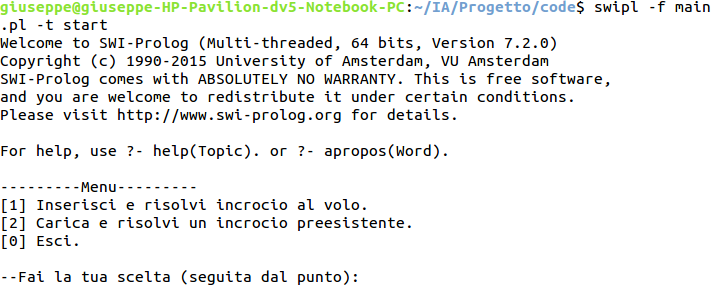
\includegraphics[width=\textwidth]{images/shell/user}
	\caption{Menu utente}
\end{figure}


\subsection{Utente amministratore}
L'utente amministratore invece ha a disposizione funzionalità più critiche:
\begin{itemize}
	\item Registrare o cancellare un incrocio nella base di conoscenza.
	\item Accedere al menu dell'utente normale.
\end{itemize}

Per registrare un nuovo incrocio è necessario inserire l'ID del nuovo esempio e la lista dei fatti che lo descrivono, separati da virgola. Per cancellarlo è necessario solamente l'ID.

\begin{figure}[!hbtp]
	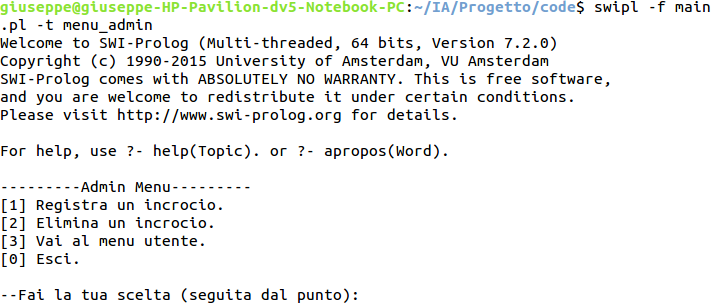
\includegraphics[width=\textwidth]{images/shell/admin}
	\caption{Menu amministratore}
\end{figure}

\section{Topologia}
Esistono quattro moduli che descrivono e gestiscono come i veicoli ed i bracci si dispongono sull'incrocio e come si relazionano gli uni con gli altri da un punto di vista logistico, e sono \texttt{destra}, \texttt{adiacenza}, \texttt{opposti} e \texttt{movimento}.

\subsection{Destra}
\label{ssec:right}
Il modulo descrive che cosa si intende quando un veicolo è a destra di un altro, o quando un braccio è a destra di un altro. Vengono utilizzati i punti cardinali visti nell'immagine \ref{fig:rose}, per definire la relazione \texttt{subito\_a\_destra/2}, ad esempio:
\begin{verbatimtab}
subito_a_destra(braccio(nord), braccio(nord_est)).
subito_a_destra(braccio(nord_est), braccio(est)).
subito_a_destra(braccio(est), braccio(sud_est)).	
\end{verbatimtab}

La relazione \texttt{destra\_lasca/2} rappresenta una concezione più ampia di destra, dove un braccio è a destra di un altro se esistono al più tre livelli di profondità di \texttt{subito\_a\_destra/2} tra bracci intermedi. Per chiarire si osservi la figura:

\begin{figure}[htb]
	\centering
	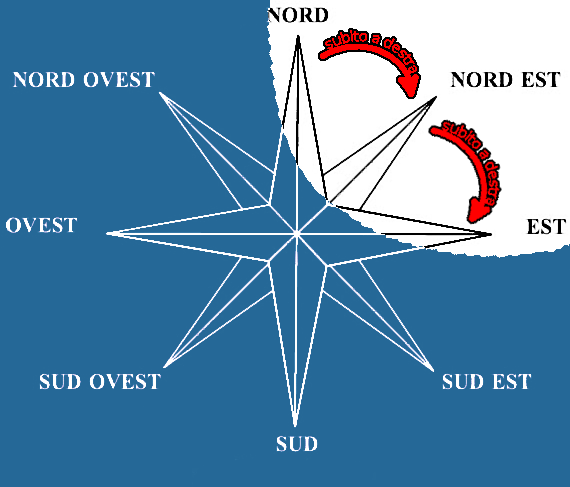
\includegraphics[width=.8\textwidth]{images/right}
	\caption{Destra lasca}
	\label{fig:right}
\end{figure}

\clearpage 
In essa si nota come il nord sia subito a destra di nord-est e come quest'ultimo sia subito a destra di est, sempre dal punto di vista del guidatore che si ferma al braccio corrispondente al punto cardinale. La zona bianca rappresenta esattamente la destra lasca, che descrive, transitivamente, che il nord è a destra di est (in modo lasco), come anche nord-est. Nella fattispecie il codice risulta:

\begin{verbatimtab}
destra_lasca(Braccio1, Braccio2) :-
	subito_a_destra(Braccio1, Braccio2).

destra_lasca(Braccio1, Braccio2) :-
	subito_a_destra(Braccio1, BraccioIntermedio),
	subito_a_destra(BraccioIntermedio, Braccio2).

destra_lasca(Braccio1, Braccio2) :-
	subito_a_destra(Braccio1, BraccioIntermedio1),
	subito_a_destra(BraccioIntermedio1, BraccioIntermedio2),
	subito_a_destra(BraccioIntermedio2, Braccio2).
\end{verbatimtab}

La relazione \texttt{da\_destra/2} invece descrive quando un \underline{veicolo} è a destra di un altro.


\subsection{Adiacenza}
La relazione \texttt{adiacente/2} riguarda i bracci dell'incrocio. Analogamente a \texttt{destra\_lasca/2}, un braccio è adiacente ad un altro se esistono al più due livelli di collegamento diretto tra bracci intermedi. Esiste quindi \texttt{collegato/2} che indica se un braccio comunica direttamente con un altro, alla sua destra o alla sua sinistra. Ad esempio:
\begin{verbatim}
collegato(braccio(est), braccio(sud_est)).
collegato(braccio(sud), braccio(sud_ovest)).
\end{verbatim}

Inoltre, \texttt{adiacente/2} è simmetrica: se il braccio A è collegato/adiacente al braccio B, allora il braccio B è collegato/adiacente al braccio A. Infatti:

\begin{verbatimtab}
adiacente(braccio(X), braccio(Y)) :-
	collegato(braccio(X), braccio(Y)).

adiacente(braccio(X), braccio(Y)) :-
	collegato(braccio(Y), braccio(X)).

adiacente(braccio(X), braccio(Y)) :-
	collegato(braccio(X), braccio(Z)),
	collegato(braccio(Z), braccio(Y)).

adiacente(braccio(X), braccio(Y)) :-
	collegato(braccio(Y), braccio(Z)),
	collegato(braccio(Z), braccio(X)).
\end{verbatimtab}

\subsection{Opposti}
La relazione \texttt{opposto/2} è simile nello spirito a destra lasca: non riguarda solo i bracci direttamente opposti, ma anche quelli che si aprono a ventaglio davanti ad un braccio, ad esempio, nel nostro contesto, il braccio nord è opposto a sud, sud-ovest e sud-est. Di conseguenza, occorre definire una relazione \texttt{di\_fronte/2} che indica quando un braccio è di fronte ad un altro e appunto, \texttt{opposto/2}, che è simmetrica. Uno stralcio di codice si presenta come:

\begin{verbatimtab}
di_fronte(braccio(nord), braccio(sud)).
di_fronte(braccio(nord), braccio(sud_est)).
di_fronte(braccio(nord), braccio(sud_ovest)).

opposto(braccio(X), braccio(Y)) :-
	di_fronte(braccio(X), braccio(Y)).

opposto(braccio(X), braccio(Y)) :-
	di_fronte(braccio(Y), braccio(X)).
\end{verbatimtab}

\subsection{Movimento}
\label{ssec:pos}
Questo modulo contiene operatori che descrivono situazioni particolari in cui i veicoli possono incrociarsi, dimostrandosi utili per la risoluzione dell'incrocio. Nello specifico essi sono:

\begin{itemize}
	\item \texttt{incrocia/2}: controlla che un veicolo ne trovi un altro nel corso della sua manovra. Sfrutta tutti i predicati elencati successivamente, insieme ad altri importati da altri moduli.
	
	\item \texttt{svolta\_a\_u/2}: si riferisce al caso in cui il braccio di arrivo di un veicolo è a destra del braccio di provenienza di un altro. Questo può comportare il caso in cui un veicolo proveniente da destra ma che dà la precedenza ad un altro si diriga in un braccio svoltando ad U.
	
	\item \texttt{transitano\_stesso\_braccio/2}: entrambi i veicoli si dirigono nella stessa direzione.
	
	\item \texttt{entrambi\_dritto/2}: copre il caso in cui i veicoli proseguono dritto, evitando di andare l'uno nel braccio nell'altro, altrimenti non potrebbero incrociarsi.
	
	\item \texttt{entrambi\_a\_sinistra/4}: ambedue i veicoli vanno a sinistra; oltre ai due veicoli, gli altri argomenti sono i bracci di destinazione.
	
	\item \texttt{uno\_a\_sinistra/4}: meno restrittiva della precedente, verifica se almeno un veicolo va a sinistra.
	
	\item \texttt{nel\_braccio\_dell\_altro/2}: un veicolo si dirige nel braccio di provenienza dell'altro.
	
	\item \texttt{dove\_vado\_uguale\_dove\_vieni/2}; I veicoli vanno reciprocamente nei bracci di provenienza dell'altro.
\end{itemize}

Il predicato \texttt{incrocia/2} viene usato solo da \texttt{precede\_da\_destra/2} del modulo \texttt{precedenze.pl}:

\begin{verbatimtab}
precede_da_destra(V1, V2) :-
	da_destra(V1, V2),
	incrocia(V1, V2),
	\+ svolta_a_u(V1, V2).
\end{verbatimtab}

Un veicolo ha la precedenza a destra rispetto ad un altro se il primo proviene da un braccio a destra di quello del secondo (cfr. \ref{ssec:right}), se lo incrocia e se non compie una svolta ad U. Per chiarire si osservi l'immagine:

\begin{figure}[!htb]
	\centering
	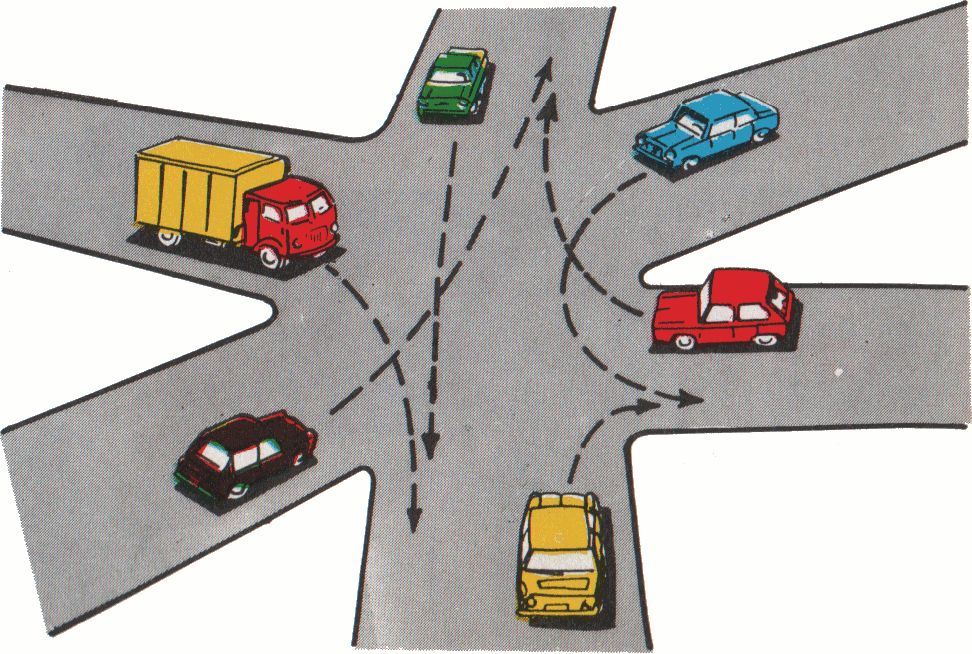
\includegraphics[width=.5\textwidth]{images/movement/uturn}
	\caption{Il veicolo celeste compie una svolta a U}
\end{figure}

Il veicolo giallo incrocia il veicolo celeste nel braccio sud-est, senza il vincolo della svolta ad U risulterebbe che, reciprocamente, uno ha la precedenza sull'altro.
\\\\
\indent Gli altri predicati usati da \texttt{incrocia/2} vengono analizzati meglio di seguito:
\begin{center}
	\begin{longtabu} to \textwidth {lX}
		\adjustbox{raise=-2.5cm}{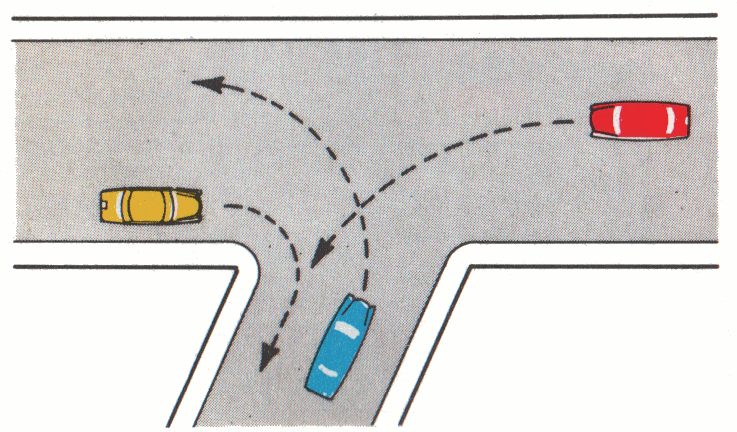
\includegraphics[width=.4\textwidth]{images/movement/same_dir}} & I veicoli rosso e giallo vanno entrambi nel braccio sud. Viene sfruttato \texttt{transitano\_stesso\_braccio/2}.\\
		
		\adjustbox{raise=-2.1cm}{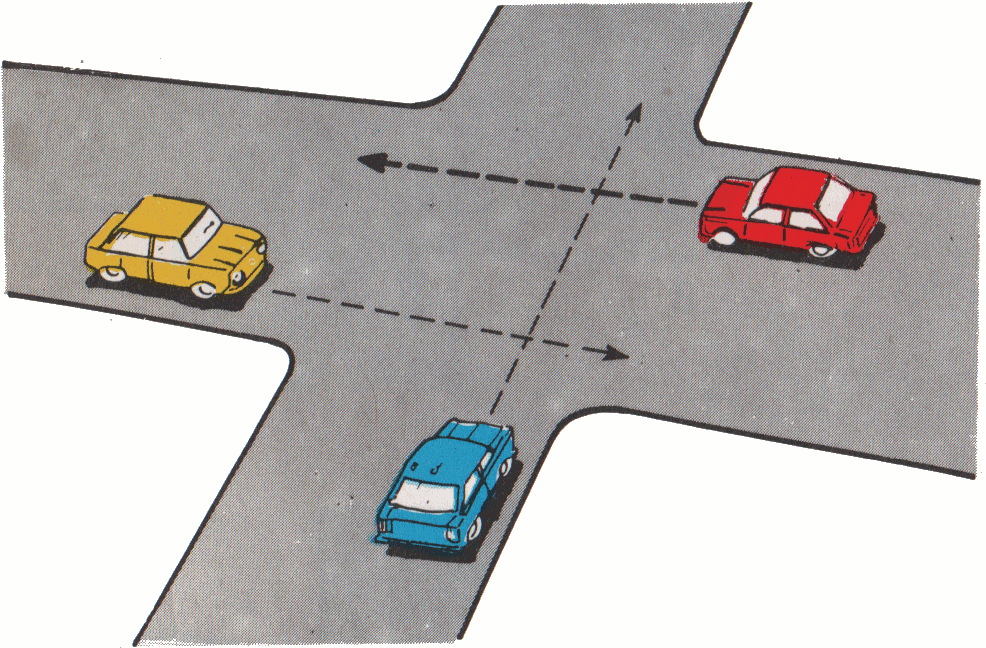
\includegraphics[width=.4\textwidth]{images/movement/both_straight}} & I veicoli rosso e celeste vanno entrambi dritto e il primo è a destra del secondo. Viene sfruttato \texttt{entrambi\_dritto/2}.\\
		
		\adjustbox{raise=-3cm}{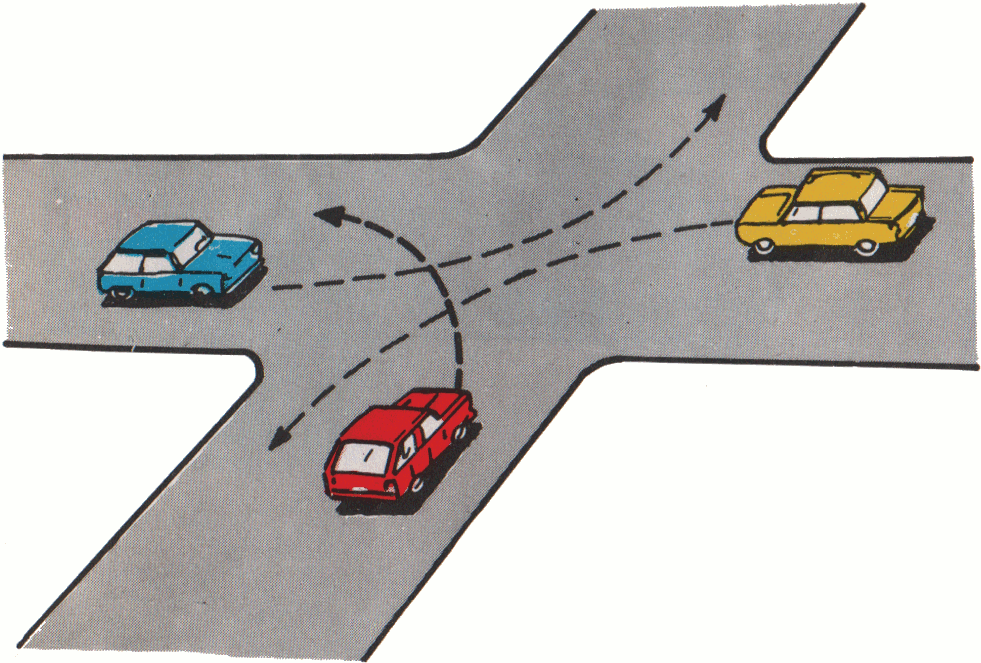
\includegraphics[width=.4\textwidth]{images/movement/both_left}} & I veicoli rosso e giallo vanno entrambi a sinistra, i bracci di provenienza sono adiacenti, così come i bracci di arrivo.   Lo stesso discorso vale per i veicoli rosso e blu. In questo caso viene utilizzato \texttt{entrambi\_a\_sinistra/4}\\
		
		\adjustbox{raise=-2.9cm}{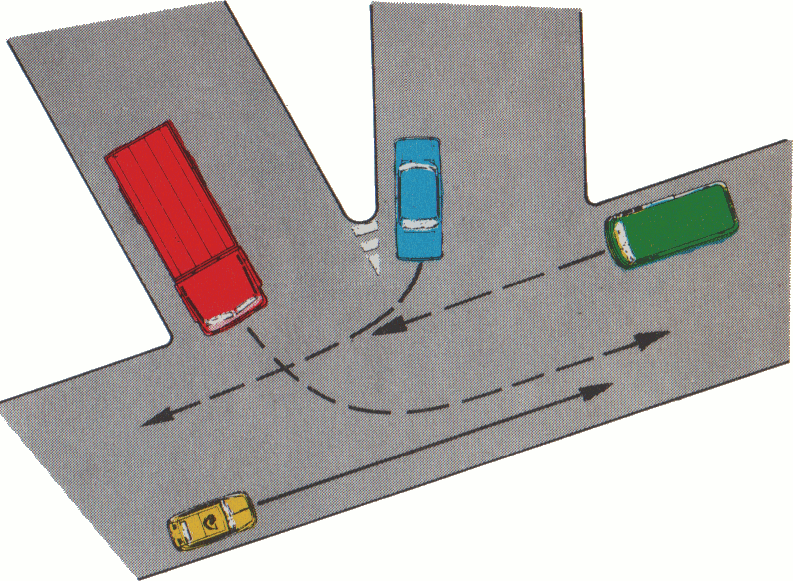
\includegraphics[width=.4\textwidth]{images/movement/one_left}} & Il camion va a sinistra mentre il veicolo celeste va a destra, proseguendo in bracci opposti. Viene sfruttato \texttt{uno\_a\_sinistra/4}. \\
		
		\adjustbox{raise=-6.45cm}{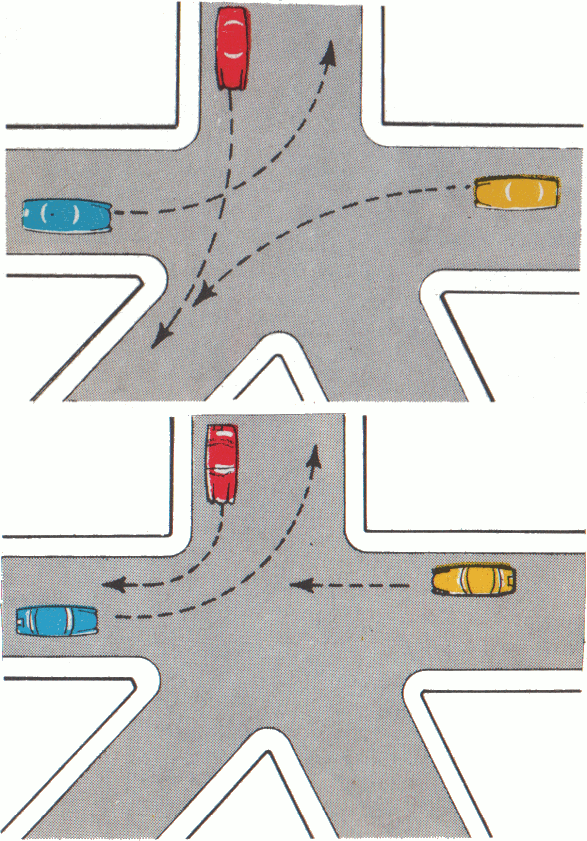
\includegraphics[width=.4\textwidth]{images/movement/mirror}} & La prima figura mostra il veicolo celeste e rosso che si incrociano, con il veicolo celeste andare a sinistra nel braccio di provenienza del rosso, assicurandoci che il rosso non faccia lo stesso, altrimenti si verificherebbe la situazione della seconda figura, dove i due veicoli non si incrociano. Nel caso della prima figura si usano \texttt{uno\_a\_sinistra/4}, \texttt{nel\_braccio\_dell\_altro/2} e \texttt{dove\_vado\_uguale\_dove\_vieni/2}.
	\end{longtabu}
\end{center}

\section{Analisi dei veicoli}
\label{sec:an}
Il modulo \texttt{analisi.pl} serve a dettagliare lo stato dei veicoli dopo che un incrocio è stato risolto. Viene chiesto all'utente (tramite prompt a riga di comando o interagendo con l'interfaccia grafica) se vuole avere ulteriori dettagli su tutti i veicoli coinvolti nell'incrocio o solamente su di uno. Le informazioni riguardano quali veicoli precedono, quali vengono preceduti e quali eventualmente si spostano insieme al veicolo in esame:

\begin{figure}[!htb]
	\centering
	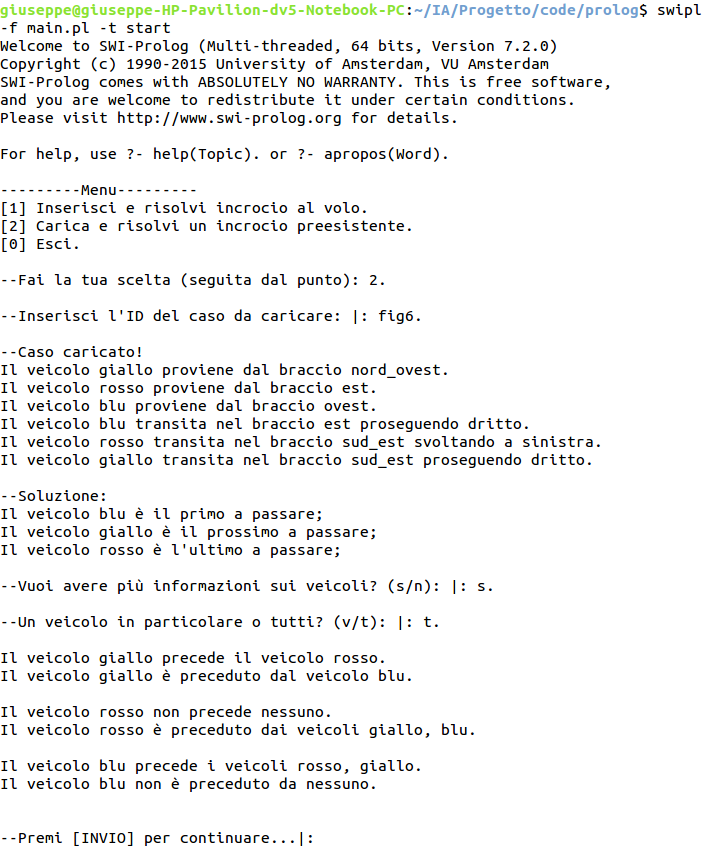
\includegraphics[width=.9\textwidth]{images/shell/info2}
	\caption{Tutti i veicoli}
\end{figure}

\begin{figure}[!htb]
	\centering
	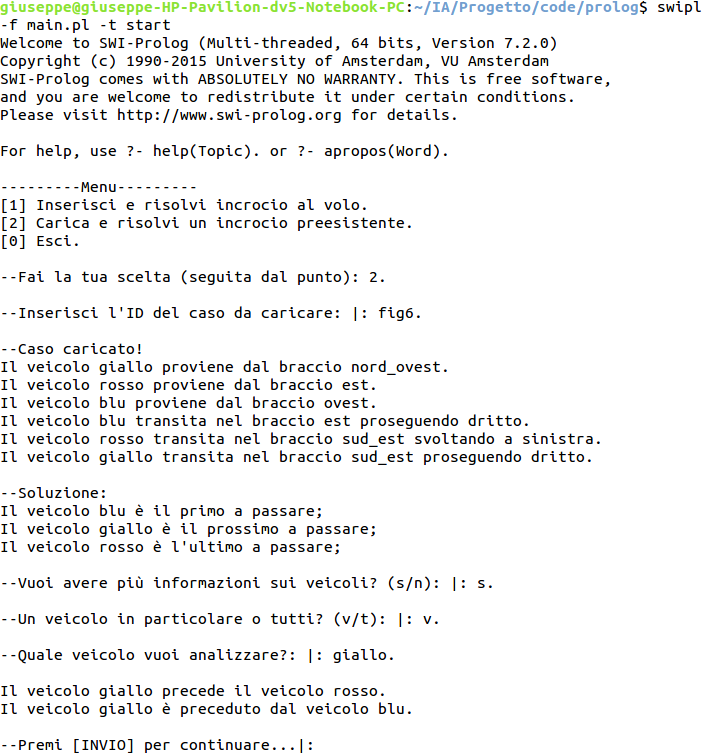
\includegraphics[width=.9\textwidth]{images/shell/info3}
	\caption{Veicolo specifico}
\end{figure}

\clearpage

Mentre se non si volessero ulteriori informazioni, si tornerebbe al menu utente:

\begin{figure}[!htb]
	\centering
	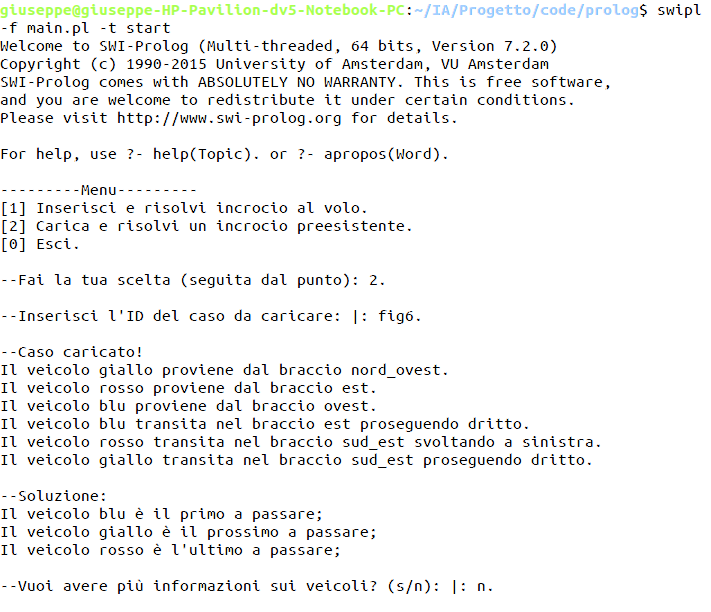
\includegraphics[width=.9\textwidth]{images/shell/info1}
	\caption{Risoluzione}
\end{figure}


\section{Accesso alla base di conoscenza}
Per potere acceder alla base di conoscenza, il file \texttt{kb.pl}, è stato realizzato il modulo \texttt{gestore\_kb.pl} che fornisce degli operatori a supporto di task di lettura e scrittura sulla memoria secondaria. I più importanti sono:
\begin{itemize}
	\item \texttt{registra\_incrocio/2}: permette ad un amministratore di sfruttare i due argomenti, l'ID e la lista dei fatti che descrivono l'incrocio, per memorizzare un nuovo oggetto \texttt{incrocio/2} nella base di conoscenza.
	\item \texttt{elimina\_incrocio/1}: cancella un incrocio in modo persistente in base all'ID.
	\item \texttt{recupera\_incrocio/2}: ritrova l'incrocio con l'ID ottenuto e lo passa a \texttt{carica\_in\_memoria/1}.
	\item \texttt{carica\_in\_memoria/1}: disseziona la lista dei fatti che descrivono l'incrocio, aggiungendo ogni compound della lista tramite \texttt{assert/1}.
	\item \texttt{pulisci/0}: una serie di \texttt{retractall/1} per rimuovere i fatti dalla memoria.
\end{itemize}

\section{Miglioramento dell'interazione}
Il programma con interfaccia grafica è nato per facilitare l'interazione con utenti che non sono avvezzi alla riga di comando e preferiscono magari un approccio più vicino a loro. Il programma è scritto in Java 1.8 e la libreria usata per l'interconnessione con SWI-Prolog si chiama InterProlog.

\subsection{Componenti}
Le componenti del software in Java sono:

\begin{itemize}
	\item Il package \texttt{gui}, che contiene le classi necessarie per costruire l'interfaccia grafica, a sua volta suddiviso in \texttt{user} e \texttt{admin} che si dividono le classi relative alle varie funzionalità a loro disposizione, come spiegato in \ref{sec:users}. Un altro subpackage è \texttt{redirector}, che contiene classi che si occupano del ridirezionamento dell'ouput nelle opportune aree di testo del programma Java.
	\item il package \texttt{prolog} che contiene le classi per gestire la comunicazione con Prolog e la validazione dei predicati scritti nel programma Java.
\end{itemize}

\begin{figure}[!htbp]
	\centering
	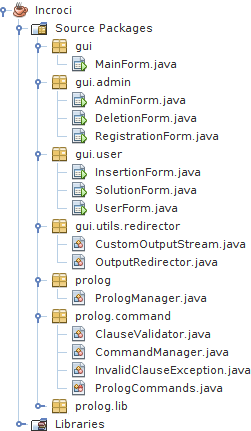
\includegraphics[width=.4\textwidth]{images/java}
	\caption{Componenti}
\end{figure}

\clearpage
Le viste implementate rispecchiano in generale l'interfaccia a menu della riga di comando, con qualche cambiamento. La prima scelta che viene posta all'utente quale a quale menu accedere, se utente o amministratore:

\begin{figure}[!htbp]
	\centering
	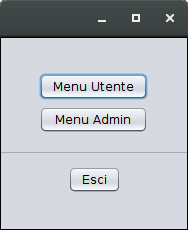
\includegraphics[width=.3\textwidth]{images/gui/menu_gui}
	\caption{Vista iniziale}
\end{figure}

In seguito verrà visualizzata una di queste due viste:
\begin{figure}[!htb]
	\centering
	\begin{subfigure}[b]{.4\textwidth}
		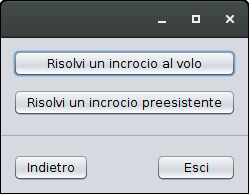
\includegraphics[width=\textwidth]{images/gui/user_gui}
		\caption{Menu Utente}
	\end{subfigure}
	\begin{subfigure}[b]{.4\textwidth}
		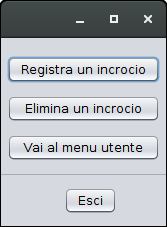
\includegraphics[width=\textwidth]{images/gui/admin_gui}
		\caption{Menu Admin}
	\end{subfigure}
	\caption{Viste dei menu}
\end{figure}

\clearpage
Per quanto riguarda il menu utente, la finestra di risoluzione di un incrocio già memorizzato è questa:
\begin{figure}[!htb]
	\centering
	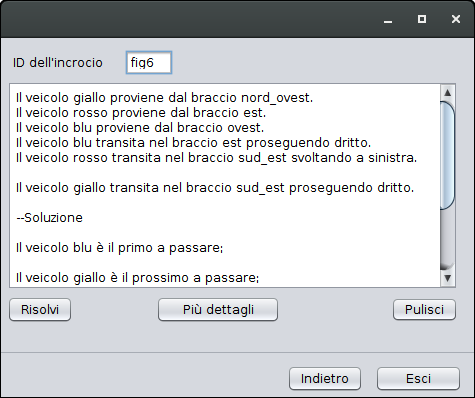
\includegraphics[width=.6\textwidth]{images/gui/solve_gui1}
	\caption{Risoluzione di un incrocio tramite ID}
\end{figure}



Se si volesse ottenere ulteriori informazioni sui veicoli dell'incrocio, come discusso in \ref{sec:an}, basterebbe premere il pulsante \adjustbox{valign=b}{
\includegraphics[scale=.7]{images/gui/more_button}} per mostrare un nuova sezione della finestra:

\newgeometry{left=1cm, right=1cm}
\begin{figure}[!htb]
	\centering
	\begin{subfigure}[b]{.4\textwidth}
		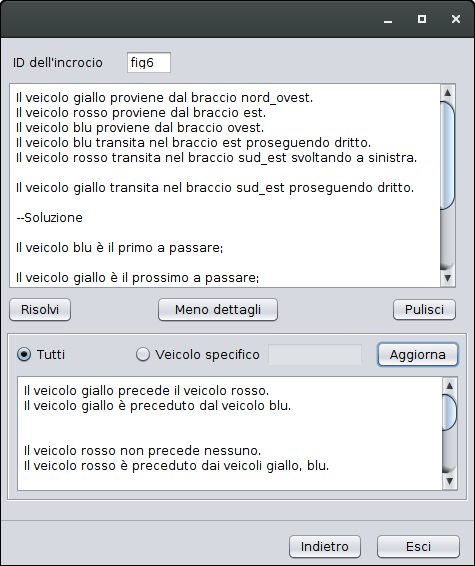
\includegraphics[width=\textwidth]{images/gui/solve_gui2}
		\caption{Tutti i veicoli}
	\end{subfigure}
	\begin{subfigure}[b]{.4\textwidth}
		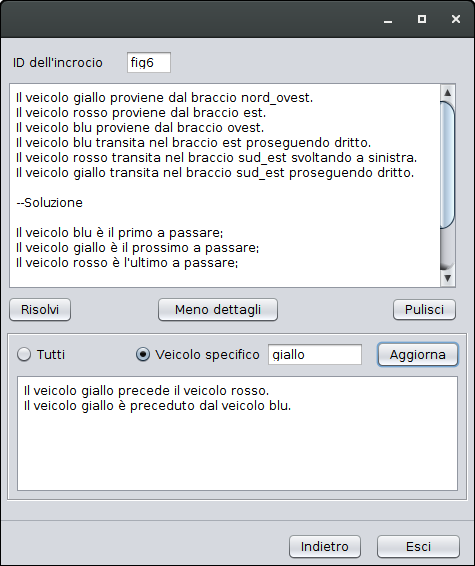
\includegraphics[width=\textwidth]{images/gui/solve_gui3}
		\caption{Veicolo specifico}
	\end{subfigure}
	\caption{Interfacce di dettaglio}
\end{figure}
\restoregeometry


Per la risoluzione di incroci che vengono inseriti direttamente dall'utente, le viste sono analoghe. Inoltre,
nel caso di inserimento di testo naturale, quindi nei due casi di incrocio che viene inserito per essere risolto \textit{on-the-fly} o memorizzato nella base di conoscenza, esso viene processato tramite espressioni regolari per ottenere i fatti nel formalismo logico appropriato.



\subsection{Bridge Java-Prolog}

La comunicazione tra Java e Prolog avviene grazie ad opportuni moduli da ambo le parti:

\begin{figure}[!htb]
	\centering
	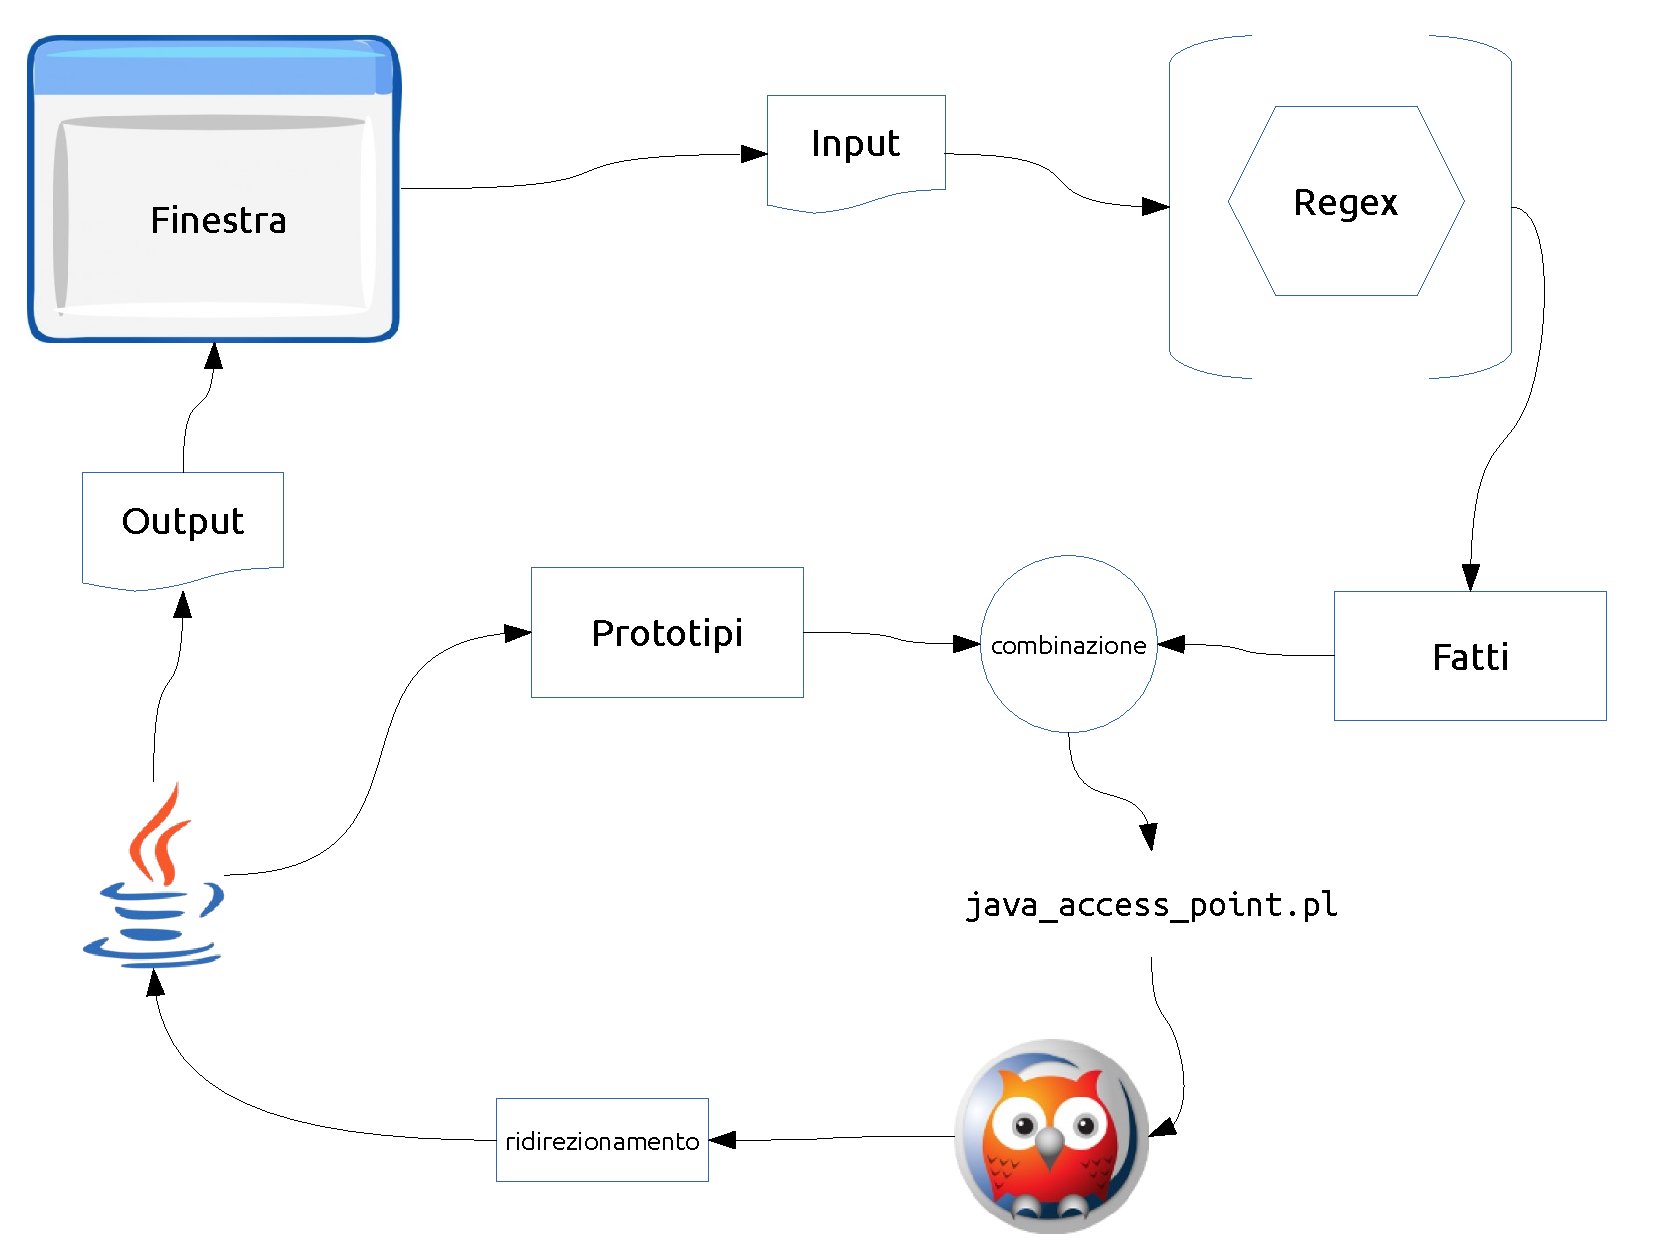
\includegraphics[width=\textwidth]{images/jap}
	\caption{Workflow della comunicazione}
\end{figure}

Di seguito viene presentata una vista generalizzata del flusso di comunicazione:
\begin{enumerate}
	\item Parte un input da una finestra del programma Java. L'input può essere testuale (i fatti che descrivono un incrocio o l'ID) o un comando (eliminazione di un incrocio).
	\item Opzionale: nel caso ci sia del testo in linguaggio naturale, esso viene processato dal modulo di validazione dei \textit{regex}, altrimenti si va direttamente al passo successivo.
	\item I fatti vengono combinati con i prototipi dei predicati (cioè i funtori dei predicati con degli argomenti segnaposto) che verranno inviati al motore Prolog.
	\item Il file \texttt{java\_access\_point.pl} è il punto di comunicazione tra Java e Prolog, che riceve i comandi che corrispondono ai prototipi inviati dal Java.
	\item Prolog viene interrogato con i comandi validati dal \texttt{java\_access\_point.pl} e risponde, restituendo un output testuale.
	\item L'output di Prolog viene intercettato e ridirezionato sull'area di testo della finestra del programma Java, chiudendo la comunicazione.
\end{enumerate}

\subsubsection{Passaggio dei dati}
\label{sssec:jap}
Il primo passo è trasformare il testo scritto dall'utente in linguaggio naturale in elementi che il Prolog possa fagocitare, quindi servono delle espressioni regolari che validino l'input che poi potrà essere convertito in compound (strutture) Prolog. Ci sono tre regex utili al nostro scopo ed ognuna descrive un tipo di fatto dell'incrocio.
La prima riguarda la provenienza del veicolo. Basandoci sull'esempio della figura \ref{fig:inc}, per descrivere il primo veicolo abbiamo: \\
\setlength{\fboxsep}{6pt}
\setlength{\fboxrule}{3pt}

\par \mbox{\fbox{\textit{Il veicolo nero proviene dal braccio ovest}}} 
%\par \noindent che diventa
\begin{flushleft}
	che diventa
\end{flushleft}
\par \mbox{\fbox{\texttt{proviene(veicolo(nero), braccio(ovest))}}}

\begin{flushleft}
	La regex utilizzata è
\end{flushleft}
\par \mbox{\fbox{\texttt{.*veicolo\textbackslash s+(.*)\textbackslash s+proviene.*braccio\textbackslash s+(.*)}}} \\\\
che valida le stringhe che contengono ``veicolo", ``proviene" e ``braccio", ignorando gli spazi e gli altri caratteri. \\


La seconda riguarda la destinazione del veicolo. Sempre basandoci sul solito esempio, per descrivere dove va il primo veicolo abbiamo: \\

\par \mbox{\fbox{\textit{Il veicolo nero transita nel braccio nord, svoltando a sinistra}}}
\begin{flushleft}
	che diventa
\end{flushleft}
\par \mbox{\fbox{\texttt{transita(veicolo(nero), sinistra, braccio(nord))}}}
\begin{flushleft}
	La regex in questo caso è:
\end{flushleft}


\setlength{\FrameSep}{6pt}
\setlength{\FrameRule}{3pt}
\begin{varwidth}{10cm}
	\begin{framed}
		\texttt{.*veicolo\textbackslash s+(.*)\textbackslash s+transita.*braccio\textbackslash  s+(.*)} \\
		\texttt{\textbackslash s+(svoltando\textbackslash s+a\textbackslash s+|proseguendo\textbackslash s+)(.*)}		
	\end{framed}
\end{varwidth} \\


che valida le stringhe che contengono ``veicolo", ``transita", ``braccio" e ``svoltando'' o ``proseguendo'', ignorando gli spazi e gli altri caratteri. \\

L'ultima riguarda la presenza di un segnale in un braccio, che ricordiamo essere opzionale. Descrivendo un segnale dell'esempio abbiamo: \\

\mbox{\fbox{\textit{Nel braccio est si trova il segnale dare\_precedenza}}}
\begin{flushleft}
	oppure
\end{flushleft}

\mbox{\fbox{\textit{Nel braccio est c'è il segnale dare\_precedenza}}}
\begin{flushleft}
	che diventa
\end{flushleft}
\par \mbox{\fbox{\texttt{si\_trova(segnale(dare\_precedenza), braccio(est))}}}

\begin{flushleft}
	La regex utilizzata è:
\end{flushleft}

\par \mbox{\fbox{\texttt{.*braccio\textbackslash s+(.*)\textbackslash s+c.*segnale\textbackslash s+(.*)}}} \\\\
che valida le stringhe che contengono ``braccio" e "segnale", ignorando gli spazi e gli altri caratteri.

Dopo aver ``spogliato" le frasi dalle parti inutili per estrarre il carico utile da inviare, c'è bisogno di richiamare i giusti operatori per interrogare Prolog. Il programma Java fornisce dei prototipi precompilati, di tipo enumerativo, che sono stringhe formattate pronte a ricevere una lista di argomenti di tipo stringa che andrà a sostituire i segnaposto presenti nel prototipo, quando ce ne sono. Questi corrispondono alle operazioni che è possibile effettuare dagli utenti e si presentano così:
\begin{itemize}
	\item \texttt{solve\_new\_crossroad(\%s)}: invocato quando si tenta di risolvere un nuovo incrocio; il segnaposto è la lista dei fatti che descrivono l'incrocio. Essa viene convertita in stringa per essere più malleabile per il Prolog.
	\item \texttt{solve\_crossroad\_by\_id(\%s)}: invocato quando si tenta di risolvere un incrocio tramite ID; il segnaposto è appunto l'ID dell'incrocio.
	\item \texttt{register\_new\_crossroad(\%s, \%s)}: invocato quando si memorizza un nuovo incrocio; i segnaposti sono l'ID dell'incrocio e la lista dei fatti che descrivono l'incrocio.
	\item \texttt{delete\_crossroad(\%s)}: invocato quando si cancella un incrocio; il segnaposto è l'ID dell'incrocio.
	\item \texttt{all\_info}: invocato quando si vogliono avere più informazioni su tutti i veicoli.
	\item \texttt{specific\_info(\%s)}: invocato quando si vogliono avere più informazioni su un veicolo specifico; il segnaposto è il veicolo.
	\item \texttt{clean}: invocato quando si vuole togliere dalla memoria l'incrocio.
\end{itemize}

Una volta combinati i prototipi con gli opportuni argomenti, essi vengono ricevuti dal modulo \texttt{java\_access\_point} che presenta gli stessi funtori dei prototipi, quindi entra in gioco Prolog che processa i dati e restituisce i risultati. Quest'ultimo semplicemente invia l'output alla riga di comando tramite \texttt{writeln/1} oppure \texttt{format/2}, che viene intercettato dal Java e ridirezionato nella finestra del programma Java.
